%----------------------------------------------------------------
%
%  File    :  thesis.tex
%
%  Authors :  Keith Andrews, IICM, TU Graz, Austria
%             Manuel Koschuch, FH Campus Wien, Austria
% 
%  Created :  22 Feb 96
% 
%  Changed :  24 March 2009
% 
%----------------------------------------------------------------

% Please send any questions, comments, remarks or complaints to
% manuel.koschuch@fh-campuswien.ac.at


% --- General Setup ---------------------------------------------

\documentclass[12pt,a4paper,oneside]{book}

%\usepackage{times}

%\renewcommand{\rmdefault}{phv} % Arial
%\renewcommand{\sfdefault}{phv} % Arial

\usepackage[utf8]{inputenc}   % so can use Umlaut chars  ä, ü

\usepackage[bf,sf]{subfigure}
\renewcommand{\subfigtopskip}{0mm}
\renewcommand{\subfigcapmargin}{0mm}

\usepackage[ngerman]{babel}         % load babel *before* natbi
%\usepackage[austrian,english]{babel}         % load babel *before* natbi
%\usepackage[square]{natbib}                  % citations


\usepackage{url}

\usepackage{latexsym}

\usepackage{ifpdf} % detect outputstyle

\usepackage{geometry} % define pagesize in more detail

\usepackage{fancyhdr} % nicer headers and footers

\usepackage{colortbl} %define colored backgrounds for tables

\usepackage{listings}

\usepackage{multicol}

\usepackage{wrapfig}

\ifpdf
  \usepackage[pdftex]{graphicx}
  \DeclareGraphicsExtensions{.pdf,.jpg,.png}
  \pdfcompresslevel=9
  \pdfpageheight=297mm
  \pdfpagewidth=210mm
  \usepackage[         % hyperref should be last package loaded
    pdftex,
    bookmarks,
    bookmarksnumbered,
    linktocpage,
    pagebackref,
    pdfview={Fit},
    pdfstartview={Fit},
    pdfpagemode=UseOutlines,                 % open bookmarks in Acrobat
  ]{hyperref}
  \usepackage{bookmark}
\else                      % latex
  \usepackage{graphicx}
  \DeclareGraphicsExtensions{.ps}
\fi

\usepackage{xcolor}


\definecolor{pblue}{rgb}{0.13,0.13,1}
\definecolor{pgreen}{rgb}{0,0.5,0}
\definecolor{pred}{rgb}{0.9,0,0}
\definecolor{pgrey}{rgb}{0.46,0.45,0.48}
\definecolor{maroon}{rgb}{0.5,0,0}
\definecolor{darkgreen}{rgb}{0,0.5,0}
\definecolor{gray}{rgb}{0.4,0.4,0.4}
\definecolor{darkblue}{rgb}{0.0,0.0,0.6}
\definecolor{cyan}{rgb}{0.0,0.6,0.6}
\definecolor{forestgreen}{RGB}{34,139,34}
\definecolor{orangered}{RGB}{239,134,64}
\definecolor{darkblue}{rgb}{0.0,0.0,0.6}
\definecolor{gray}{rgb}{0.4,0.4,0.4}
\definecolor{dkgreen}{rgb}{0,0.6,0}
\definecolor{gray}{rgb}{0.5,0.5,0.5}
\definecolor{mauve}{rgb}{0.58,0,0.82}
\definecolor{light-gray}{gray}{0.25}

\lstdefinelanguage{XML}
{
  basicstyle=\ttfamily,
  morestring=[s]{"}{"},
  morecomment=[s]{?}{?},
  morecomment=[s]{!--}{--},
  commentstyle=\color{darkgreen},
  moredelim=[s][\color{black}]{>}{<},
  moredelim=[s][\color{red}]{\ }{=},
  stringstyle=\color{blue},
  identifierstyle=\color{maroon}
}

\lstdefinestyle{SQL-Michalstyle}
{%
  language   = SQL,
  basicstyle = \fontsize{9}{13}\ttfamily,
  columns    = fixed,
  numbers    = left,
}

\lstdefinestyle{JAVA-Own}
{%
  language=Java,
  showspaces=false,
  showtabs=false,
  breaklines=true,
  showstringspaces=false,
  breakatwhitespace=true,
  numbers    = left,
  commentstyle=\color{pgreen},
  keywordstyle=\color{pblue},
  stringstyle=\color{pred},
  basicstyle=\fontsize{9}{13}\ttfamily,
  moredelim=[il][\textcolor{pgrey}]{$$},
  moredelim=[is][\textcolor{pgrey}]{\%\%}{\%\%}
}
\lstdefinestyle{sharpc}{
  language   = [Sharp]C,
  frame      = single,
  numbers    = left,
  breaklines=true,
  breakatwhitespace=true,
  basicstyle =\fontsize{9}{13}\ttfamily,
}

\lstdefinestyle{XML-Own} {
  language=XML,
  extendedchars=true, 
  breaklines=true,
  breakatwhitespace=true,
  emph={},
  emphstyle=\color{red},
  basicstyle={\footnotesize\ttfamily},
  numbers=left,
  columns=fullflexible,
  commentstyle=\color{gray}\upshape,
  morestring=[b]",
  morecomment=[s]{<?}{?>},
  morecomment=[s][\color{forestgreen}]{<!--}{-->},
  keywordstyle=\color{orangered},
  stringstyle=\ttfamily\color{black}\normalfont,
  tagstyle=\color{darkblue}\bf,
  morekeywords={attribute,xmlns,version,type,release},
}

\lstdefinestyle{csharp} {
  aboveskip=3mm,
  belowskip=3mm,
  showstringspaces=false,
  columns=flexible,
  basicstyle={\footnotesize\ttfamily},
  numbers=left,
  keywordstyle=\color{blue},
  commentstyle=\color{dkgreen},
  stringstyle=\color{mauve},
  breaklines=true,
  breakatwhitespace=true,
  tabsize=3,
  morecomment = [l]{//}, 
  morecomment = [l]{///},
  morecomment = [s]{/*}{*/},
  morestring=[b]", 
  sensitive = true,
  morekeywords = {async, await, abstract,  
    event,  new,  struct,
    as,  explicit,  null,  switch,
    base,  extern,  object,  this,
    bool,  false,  operator,  throw,
    break,  finally,  out,  true,
    byte,  fixed,  override,  try,
    case,  float,  params,  typeof,
    catch,  for,  private,  uint,
    char,  foreach,  protected,  ulong,
    checked,  goto,  public,  unchecked,
    class,  if,  readonly,  unsafe,
    const,  implicit,  ref,  ushort,
    continue,  in,  return,  using,
    decimal,  int,  sbyte,  virtual,
    default,  interface,  sealed,  volatile,
    delegate,  internal,  short,  void,
    do,  is,  sizeof,  while,
    double,  lock,  stackalloc,   
    else,  long,  static,   
    enum,  namespace,  string }
}

\lstdefinestyle{BashInputStyle}{
  language=bash,
  firstline=2,% Supress the first line that begins with `%`
  basicstyle=\small\ttfamily,
  numbers=left,
  columns=fullflexible,
  linewidth=0.9\linewidth,
  xleftmargin=0.1\linewidth
}



\geometry{a4paper,left=30mm,right=25mm, top=30mm, bottom=30mm}

\setlength{\parskip}{3pt plus 1pt minus 0pt}       % vert. space before a paragraph

\setcounter{tocdepth}{1}        % lowest section level entered in ToC
\setcounter{secnumdepth}{2}     % lowest section level still numbered


% --- Start of Document ----------------------------------------


\begin{document}

\frontmatter
\normalsize
\pagestyle{empty}            % for title pages

%----------------------------------------------------------------
%
%  File    :  title.tex
%
%  Authors :  Keith Andrews, IICM, TU Graz, Austria
%             Manuel Koschuch, FH Campus Wien, Austria
% 
%  Created :  22 Feb 96
% 
%  Changed :  24 March 2009
%  !TEX root = ./thesis.tex
%----------------------------------------------------------------


% --- Main Title Page ------------------------------------------------

% A4 paper =  w=21cm, h=29.7cm

%\setlength{\textheight}{26.83cm}
%\setlength{\textwidth}{17cm}
%
%\setlength{\oddsidemargin}{-0.04cm}
%\setlength{\topmargin}{-2.5cm}

\vspace*{-2.5cm}
\begin{center}
\end{center}

\begin{center}

\vspace{1.3cm}

\hspace*{-1.0cm} {\Large \textbf{Cross-platform development\\}}

\hspace*{-1.0cm} unter Xamarin.Forms \\

\vspace{2.2cm}

\hspace*{-1.0cm} \textbf{Bachelorarbeit 2\\}

\vspace{0.65cm}

\hspace*{-1.0cm}\\
\hspace*{-1.0cm}\\
\hspace*{-1.0cm} Angefertigt an der der \\
\hspace*{-1.0cm} Fachhochschule Campus Wien \\
\hspace*{-1.0cm} Bachelorstudiengang Informationstechnologien und Telekommunikation \\

\vspace{7cm}

\hspace*{-1.0cm} Vorgelegt von: \\
\hspace*{-1.0cm} Maximilian Hans Peter Thomas Peßl \\
\hspace*{-1.0cm} Personenkennzeichen: c1510475049 \\

\vspace{2.1cm}

\hspace*{-1.0cm} Vertiefungsrichtung: \\
\hspace*{-1.0cm} Telekommunikation\\

\vspace{0.5cm}


\vspace{1.4cm}

\hspace*{-1.0cm} Abgabetermin: 03.06.2018 \\

\end{center}

\newpage

\vspace*{17cm}

\hspace*{-0.7cm} \underline{Erklärung:}\\\\
Ich erkläre, dass die vorliegende Bachelorarbeit von mir selbst verfasst wurde und ich keine anderen als die angeführten Behelfe verwendet bzw. mich auch sonst keiner unerlaubter Hilfe bedient habe.\\
Ich versichere, dass ich dieses Bachelorarbeitsthema bisher weder im In- noch im Ausland (einer Beurteilerin/einem Beurteiler zur Begutachtung) in irgendeiner Form als Prüfungsarbeit vorgelegt habe.\\
Weiters versichere ich, dass die von mir eingereichten Exemplare (ausgedruckt und elektronisch) identisch sind.\\\\
Datum: \hspace{6cm} Unterschrift:\\






              % Title Page

\pagestyle{fancy}
\fancyhead{}
\fancyfoot{}
\setlength{\headheight}{15pt}
\renewcommand{\headrulewidth}{0.0pt}
\fancyfoot[R]{\thepage}      
\pagenumbering{roman}        % for preliminary pages

% %----------------------------------------------------------------
%
%  File    :  acknowl.tex
%
%  Authors :  Keith Andrews, IICM, TU Graz, Austria
%             Manuel Koschuch, FH Campus Wien, Austria
% 
%  Created :  22 Feb 96
% 
%  Changed :  30 Oct 2008
%  !TEX root = ./thesis.tex
%----------------------------------------------------------------

\begin{center}
{\Large\bfseries Danksagung}
\end{center}

(Falls gewünscht.)            % Acknowledgements

%----------------------------------------------------------------
%
%  File    :  abstracts.tex
%
%  Authors :  Keith Andrews, IICM, TU Graz, Austria
%             Manuel Koschuch, FH Campus Wien, Austria
% 
%  Created :  22 Feb 96
% 
%  Changed :  30 Oct 2008
%  !TEX root = ./thesis.tex
%----------------------------------------------------------------


% --- German and English Abstracts ------------------------------------------------

% --- German Abstract ----------------------------------------------------
\cleardoublepage

\begin{center}
{\Large\bfseries Kurzfassung}
\end{center}

Apple und Android sind heutzutage die größten Vertreter von mobilen Betriebssystemen und erfreuen sich stetig steigender Beliebtheit. Als Software Entwickler muss nach dem Design einer Applikation und der funktionalen Anforderungen schlussendlich eine Entscheidung über die Zielplattform getroffen werden. Diese Wahl gestaltet sich an sich sehr leicht, weil als größte Vertreter entweder Apples iOS oder Googles Android zur Verfügung stehen. Dies spiegelt den klassischen Software Engineering (SE) Prozess mit den Phasen Analyse, Design, Implementierung, Testen und Wartung wieder. Dabei ist es gegenstandslos, ob es sich um die Entwicklung einer Nativen Applikation, oder Cross-Platform (CP) Anwendung handelt. Vor allem in der Implementierung und Test Phase ist die Entwicklung symmetrisch.

Jedoch gibt es bedeutende Unterschiede in den Phasen Analyse und Design. Bei der Verwendung von Cross-Platform Frameworks (CPF) spielt die Analyse der Anforderungen und die darauf anschließende Design Phase eine beträchtliche Rolle. Xamarin.Forms ermöglicht es für die Entwicklung einer mobilen Applikation die Anwendung aus einer sehr objektiven Betrachtungsweise zu spezifizieren. Dabei ermöglicht es dem Entwickler sich auf die Funktionalitäten der Anwendung und nicht auf die zielbetriebssystemspezifischen Design Elemente zu konzentrieren. Die Arbeit befasst sich ausführlicher mit dem CPF Xamarin.Forms und wie sich die Entwicklung einer mobilen Applikation durch Anwendung eines solchen Frameworks verändert.

% --- English Abstract ----------------------------------------------------

\cleardoublepage

%\selectlanguage{english}

\begin{center}
{\Large\bfseries Abstract}
\end{center}

Apple and Android are the largest representatives of mobile operating systems today and are becoming increasingly popular. As a software developer, a decision about the target platform must finally be made after the design of an application and the functional requirements. This choice is very easy in itself because the largest representatives are either Apple's iOS or Google's Android. This reflects the classic Software Engineering (SE) process with the phases analysis, design, implementation, testing and maintenance. It is irrelevant whether it concerns the development of a native application or a Pross-Platform (CP) application. Especially in the implementation and test phases, the development is symmetrical.

However, there are significant differences in the analysis and design phases. When using Cross-Platform Frameworks (CPF), the analysis of the requirements and the subsequent design phase plays a considerable role. Xamarin.forms makes it possible for the development of a mobile application to specify the application from a very objective point of view. It allows the developer to focus on the functionalities of the application and not on the target operating system specific design elements. The work deals in more detail with the CPF Xamarin.forms and how the development of a mobile application changes through the application of such a framework.

%\selectlanguage{austrian}
          % Englisch and German abstracts

%----------------------------------------------------------------
%
%  File    :  glossary.tex
%
%  Author  :  Manuel Koschuch, FH Campus Wien, Austria
% 
%  Created :  30 Oct 2008
% 
%  Changed :  30 Oct 2008
%  !TEX root = ./thesis.tex
%----------------------------------------------------------------

\begin{center}
{\Large\bfseries Abkürzungsverzeichnis}
\end{center}

\begin{table*}[htbp]
		\begin{tabular}{ll}
			AoT &	Ahaed of Time\\
			API &	Application Programming Interface\\
			CP  &	Cross-Platform \\
			CPF &	Cross-Platform Framework \\
			IDE	&	Integrated Development Environment\\
			JIT &	Just-In-Time \\
			MAD &	Mobile App Development \\
			MVC &	Model View Controller\\
			MVVM&	Model View View Model\\
			PCL	&	Portable Class Library\\
			REST&	Representational State Transfer\\
			SA 	&	Shared Asset\\
			SE	&	Software Engineering\\
			SL	&	Shared Library\\
			UI	&	User Interface\\
			XAML&	Extensible Application Markup Language\\
		\end{tabular}
\end{table*}           % Glossary

%----------------------------------------------------------------
%
%  File    :  keywords.tex
%
%  Author  :  Manuel Koschuch, FH Campus Wien, Austria
% 
%  Created :  30 Oct 2008
% 
%  Changed :  30 Oct 2008
%  !TEX root = ./thesis.tex
%----------------------------------------------------------------

\begin{center}
{\Large\bfseries Schlüsselbegriffe}
\end{center}

\noindent
Cross-Platform\\
Cross-Platform Framework\\
Integrated Development Environment\\
Mobile App Development\\
Model View View Model\\
Representational State Transfer\\
Software Engineering\\
Xamarin\\
Xamarin.Forms\\
Xamarin.Native\\
           % Keywords

%----------------------------------------------------------------
%
%  File    :  toc.tex
%
%
%  Authors :  Keith Andrews, IICM, TU Graz, Austria
%             Manuel Koschuch, FH Campus Wien, Austria
% 
%  Created :  22 Feb 96
% 
%  Changed :  30 Oct 2008
%  !TEX root = ./thesis.tex
%----------------------------------------------------------------

{
\setlength{\parskip}{3pt plus 3pt minus 3pt}     % compact table of contents

\tableofcontents
}
                % Table of Contents

\mainmatter

\cleardoublepage
\renewcommand{\headrulewidth}{0.4pt}
\pagestyle{fancy}            % for main pages
\fancyhead[RO]{\slshape \nouppercase{\leftmark}}
\fancyfoot[R]{\thepage}   
\pagenumbering{arabic}      % for main pages

%--- Include your chapters here ----------

%----------------------------------------------------------------
%
%  File    :  chapter1.tex
%
%  Authors :  Keith Andrews, IICM, TU Graz, Austria
%             Manuel Koschuch, FH Campus Wien, Austria
% 
%  Created :  22 Feb 96
% 
%  Changed :  24 March 2009
%  !TEX root = ./thesis.tex
%----------------------------------------------------------------

\chapter{Einführung}
\label{chap:intro}
	Mobile App Development (MAD) und Software Engineering (SE) sollen den Entwicklungsprozess einer Software oder Mobilen Applikation insofern erleichtern, dass durch klar definierte Phasen der Entwicklungsprozess dokumentiert und verstanden wird \cite{Anthony2010}. Die Phasen bei SE beginnen mit der Analyse der Anforderungen an die zu entwickelnde Applikation. Durch gezielte Fragen und Diskussionen mit dem Kunden wird versucht ein erstes Bild von dem zu schaffen was nach Abschluss der Entwicklung der breiten Masse an Anwendern zur Verfügung gestellt werden soll. Anschließend wird es in der Design Phase spezifischer. In dieser Phase geht es nicht primär um das Aussehen und die Darstellung der unterschiedlichen User Interface (UI) Elemente sondern auch um die Spezifizierung der funktionalen und nicht funktionalen Anforderungen an die Anwendung \cite{Anthony2010}. Anschließend folgt die Phase der Implementierung gefolgt von einer Test Phase. Die Software geht anschließend an den Kunden bzw. an die Smartphone Anwender wenn es sich um eine Applikation handelt und wird in der Wartungsphase, im normal Fall einer kontinuierlichen Weiterentwicklung unterzogen. In der Wartungsphase geht es um die Behebung von \textit{Bugs} (Anwendungsfehler die einen Absturz der Applikation oder das Verwenden der Applikation erheblich erschweren), welche während der Testphase nicht gefunden wurden. 

	Diese Arbeit beschäftigt sich hauptsächlich mit den beiden ersten Phasen von SE und der Implementierung unter Xamarin.Forms als Cross-platform Framework. Xamarin und im besonderen Xamarin.Forms werden in Abschnitt \ref{chap:xamarin} genauer erläutert. Abschnitt \ref{chap:xamarin} bildet die Grundlage zu verstehen wie die Entwicklung mit einem CPF funktioniert und welche Überlegungen notwendig sind eine Applikation mit eben jenem Framework zu entwickeln.

	Jene Überlegungen die vor der Implementierung oder der ersten Programmierung von Funktionen der Applikation getroffen werden müssen, sind die Basis folgender Fragestellung mit welcher sich die Arbeit im zentralen beschäftigen wird:\vspace{1cm}

	\textit{Welche Einschränkungen ergeben sich durch Xamarin.Forms als Cross-platform Framework, im Vergleich zu Nativer Applikationsentwicklung unter Android und Cross-platform Entwicklung unter Xamarin.Native}?

\section{Motivation}
\label{sec:motivation}

	Smartphones haben heutzutage einen wichtigen Bestandteil des täglichen Lebens eingenommen. Der kurze Blick auf das Smartphone, auf dem Weg in die Schule oder in die Arbeit, sind Teil einer täglichen Routine geworden. Die Informationsbeschaffung ist durch mobiles Internet wie LTE (Long Term Evolution oder auch 4G) und immer schneller werdenderer Prozessoren in Smartphones einfacher denn je geworden. Doch nicht nur die Hardware der Anwender befindet sich in einem stetigen Prozess der Weiterentwicklung sondern auch die darauf laufende Software wie das Betriebssystem und diverse Applikationen. Apples iOS befindet sich derzeit in der Version 11.2.6 und wird bald Version 11.3.3 veröffentlichen. Im Vergleich dazu ist Android in Version 8.1.0 auf den aktuellsten Geräten bereits vorinstalliert. Apple begann mit seinem mobilen Betriebssystem iOS im Jahre 2005 und veröffentlichte 2007 iOS in der Version 1.0.x. Google begann 2008 seinen Start mit Android in der Version 1.0, auch bekannt als API 1. Seit der Einführung beider Betriebssysteme hat sich in den Jahren bis 2017 einiges getan. Gab es zu Beginn des Ersten Quartals 2009 noch folgende Vertreter:
	\begin{itemize}
		\setlength\itemsep{0em}
		\item Google - Android
		\item Apple - iOS
		\item Microsoft - Windows
		\item RIM - Blackberry
		\item Nokia - Symbian
	\end{itemize}

	Sind aktuell nur iOS und Android mit weltweiten Marktanteilen von 87,7\% für Android und 12,1\% für iOS übrig geblieben. Dies ist in Abbildung \ref{fig:mobile-os-marketshares} zu erkennen.

	Durch kontinuierliche Weiterentwicklung von Android und iOS erreichten diese eine immer größer werdende Beliebtheit wodurch andere Betriebssysteme weitgehend an Bedeutung verloren haben und schlussendlich keinen nennenswerten Anteil laut heutigen Statistiken besitzen.

	Jedoch sollte als Ausnahme die Firma RIM mit dem Betriebssystem BlackBerry OS erwähnt werden. Seit Blackberry OS 10 wurde es möglich Android Anwendungen ausführen zu können. Dies erzielte zwar nicht den erhofften Erfolg, war jedoch eine Besonderheit. Die Möglichkeit Anwendungen eines anderen Betriebssystems, wie zum Beispiel Android, installieren und auf die gleiche Art und Weise verwenden zu können ermöglichte es Anwendern, die Blackberry aufgrund seines außergewöhnlich Sicherheitsorientierten Betriebssystems verwendeten, das Beste aus beiden Welten zu vereinen.

	\newpage
	
	\begin{figure}[h!]
		\centering
		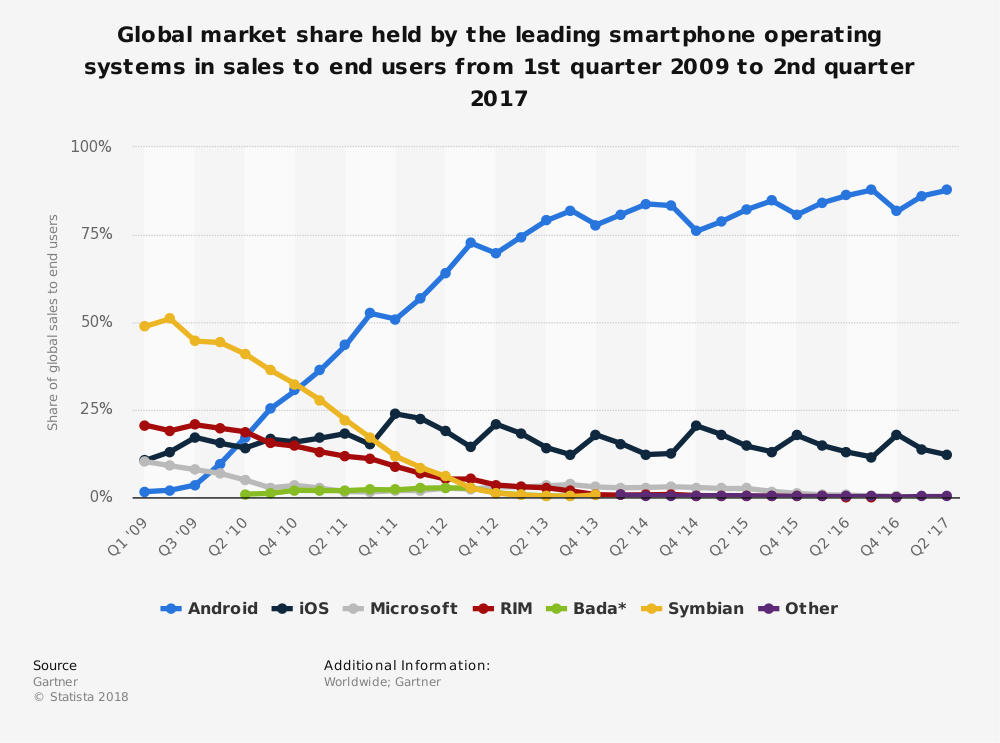
\includegraphics[width=1\textwidth]{images/statistic_id266136_global-mobile-os-market-share-2009-2017-by-quarter.png}
		\caption{Weltweiter Marktanteil an Mobilen Betriebssystemen von 2007 bis 2017 Stand Q1 2018 (Quelle: https://www.statista.com/statistics/266136/global-market-spare-held-by-smartphone-operating-systems/)}
		\label{fig:mobile-os-marketshares}
	\end{figure}
	Android ist aus heutiger Sicht das beliebteste Betriebssystem im weltweiten Vergleich. Doch warum finden sich in beiden App Stores, Google Play für Android und App Store für Apple, weit mehr als 2.000.000 Applikationen, wobei Android mit 3.361.843\footnote{https://de.statista.com/statistik/daten/studie/208599/umfrage/anzahl-der-apps-in-den-top-app-stores/} Anwendungen um mehr als 30\% mehr Applikationen als iOS zur Verfügung stellt. Diese Differenz scheint auf den Ersten Blick enorm, jedoch gilt es dabei folgenden Unterschied zu beachten. Applikationen können unter Android einfacher entwickelt und veröffentlicht werden. Apple zieht hier eine Grenze und gibt bestimmte Vorgaben vor und überprüft Apps genauer als Google. Weiters benötigt man einen Apple Developer Zugang der mit jährlichen Kosten verbunden ist.

	\newpage
	Die Motivation eine Cross-platform Applikation zu entwickeln ruht meist auf der Überlegung, warum man eine Applikation zwei Mal entwickeln muss, wenn sich eigentlich nur das Aussehen der Applikation verändert, nicht aber die grundlegenden Funktionalitäten \cite{Maximilian2017}. Als Beispiel dient die Facebook App die sowohl für Android als auch iOS mit React Native programmiert wurde. Demnach steht eine Vielzahl an CPF's der unterschiedlichsten Hersteller zur Verfügung.

	Folgende sind die populärsten \footnote{https://medium.com/@MasterOfCodeGlobal/best-10-android-frameworks-for-building-android-apps-d2d0ee48e464}:
	\begin{itemize}
		\setlength\itemsep{0em}
		\item Corona SDK - Spiel und Mobile App Development
		\item Xamarin
		\item Appcelerator Titanium
		\item React Native
		\item PhoneGap
		\item Iconic
		\item Sencha Touch
	\end{itemize}

	Alle CPF's bieten auf unterschiedlichste Art und Weise die Möglichkeit Applikationen auf Basis des \grqq Shared Codes\grqq, gemeinsame Funktionalitäten zusammenzufassen und nur einmal implementieren zu müssen. Der in der Integrierten Development Environment (IDE) eingebaute Compiler übernimmt die Aufgabe den Code entsprechend so zu kompilieren, damit dieser auf der Zielplattform nativ ausgeführt werden kann.

\newpage
\section{Related Work}
\label{sec:relatedwork}

Im Zuge der Literatur Recherche befassen sich einerseits, eine Vielzahl an Artikeln, Bachelor oder Master Arbeiten mit den Stärken und Schwächen von Cross-platform Frameworks, andererseits jedoch mit sehr spezifischen Themen der Applikationsentwicklung wie zum Beispiel Responsive UI Elements oder die Unterschiede wie ein Layout mit dem notwendigen Code dahinter interagiert und verknüpft wird. Dabei wird wiederum im speziellen auf die Kommunikation zwischen Layout und Code geachtet und analysiert.

Die Bücher \cite{book:Xamarin.Forms-Succinctly}, \cite{book:Xamarin.Forms-Essentials:} und \cite{book:Cross-platform-UI-Development-with-Xamarin.Forms} dienen als Grundlage um den Prozess der Implementierung einer Applikation mit der IDE zu verstehen und zu üben. Weiters gab es zwei Online Kurse um das in den Büchern erlernte Wissen praktisch umzusetzen.

Oleksandr Gridin widmet sich in seiner Bachelor Arbeit \cite{Oleksandr2015}, dem Xamarin Framework um dessen Stärken und Schwächen, anhand einer Android und Windows (Universal Windows Platform (UWP)) Applikation zu zeigen. Dabei wird sehr auf den Aufbau des Xamarin Frameworks, unter anderem auch Xamarin.Forms eingegangen. Im Zuge seiner Entwicklung ist es immer wieder zu Schwierigkeiten gekommen weil es keine oder nur wenige Komponenten gab um diverse Funktionalitäten umzusetzen.

In seiner Arbeit \cite{Armgren852125} \textit{Mobile Cross-platform development versus native development} widmet sich Armgren Marc, der  Performance von Xamarin als Cross-platform Framework in Bezug auf UI und Netzwerk Verkehr im Vergleich zu Nativer Applikations Entwicklung. Dabei wurden die Unterschiede zwischen Nativen iOS und Android und deren Cross-platform Pendant herangezogen. Die Evaluierung ergab das erst dann entschieden werden kann ob ein CPF verwendet werden soll wenn die Anforderungen klar definiert sind. Applikationen die eine Vielzahl an schwierigen Berechnungen durchführen müssen, wie zum Beispiel Spiele, profitierten von Nativen Code, da dieser performanter auf dem Zielbetriebssystem interpretiert und ausgeführt werden kann. In Bezug auf die Netzwerk Performance wurden keine Unterschiede festgestellt. 

Die Autoren V. Bhuttoo und K. Soman und R. K. Sungkur behandeln in dem Artikel \cite{8016193} die Stärken und Schwächen von Xamarin und stellen diese anderen bekannten Cross-platform Frameworks gegenüber. Dabei bedienten sie sich CPF's wie PhoneGap, verwendet HTML/CSS und Javascript um CP Apps zu entwickeln, und Titanium welches nur Javascript verwendet. Weiters beschäftigt sich dieser Artikel mit der Installation von CPF's und Komponenten des NuGET Paket Managers. Ihre Erkenntnisse zeigen das es überaus wichtig ist zu wissen welche Technologien Cross-platform Frameworks verwenden und wie man diese bestmöglich für eine CP App verwenden kann.

Die Arbeit von Ilke Soylemez \cite{Mukesh2016} erklärt wie die Entwicklung einer Cross-platform Applikation anhand eines Beispiels abläuft. Dabei wird vor allem auf essentielle Bausteine des Xamarin Frameworks eingegangen. Diese Bausteine sind unter anderem die Verwendung einer PCL (Portable Class Library) die, für die gemeinsame Geschäftslogik statt einer Shared Library, den Code der Cross-platform App implementiert. Weiters wird auf das MVVM (Model View View Model) Design Pattern von Xamarin eingegangen und wie dieses das Layout den notwendigen \textit{Code behind} implementiert. Allerdings wird sich weitgehend mit Xamarin.Native befasst wobei das MVVM Design Pattern sowohl bei Xamarin.Native als auch bei Xamarin.Forms zum Einsatz kommt.

In meiner vorigen Arbeit zum Thema Cross-platform Development \cite{Maximilian2017} wurde die Entwicklung einer Cross-platform Applikation auf Basis einer Nativen Applikation betrachtet. Dabei ging es vorrangig um Xamarin als CPF und welche Unterschiede oder Schwierigkeiten bei der Entwicklung einer Cross-platform App im Vergleich zu Nativer Applikationsentwicklung auftreten. Dabei wurde eine in JAVA unter Android Studio entwickelte Applikation erneut spezifiziert und unter Xamarin.Native für Android und iOS implementiert. Im Zuge der erneuten Anforderungsanalyse und Design Phase konnten während der Implementierung einige Zeilen an Code eingespart werden, da Xamarin Komponenten beispielsweise für eine Kommunikation mit einer SQL Datenbank zur Verfügung stellt in die PCL Klasse ausgelagert werden wodurch diese Kommunikation mit einem Server nur einmal implementiert werden musste. Beide Applikationen konnten durch aufrufen der Funktionen den selben Code ausführen. Allerdings verlangte Xamarin.Native das Design der App zweimal zu Entwickeln, was einen enormen Programmieraufwand verlangte.
          % Introduction

%----------------------------------------------------------------
%
%  File    :  chapter2.tex
%
%  Authors :  Keith Andrews, IICM, TU Graz, Austria
%             Manuel Koschuch, FH Campus Wien, Austria
% 
%  Created :  22 Feb 96
% 
%  Changed :  30 Oct 2008
%  !TEX root = ./thesis.tex
%----------------------------------------------------------------


\chapter{Xamarin als Cross-Platform Framework}
\label{chap:xamarin}
	Xamarin ist ursprünglich als Firma Xamarin 2011 von Mono Entwicklern gegründet und 2016 von Microsoft übernommen worden. Microsoft hat Xamarin weiterentwickelt und stellt es heute als Open-Source Cross-platform Framework für Visual Studio ab Version 2015 und für Mac als Visual Studio for Mac zur Verfügung. Mit diesem Framework kann eine Cross-platform Applikation für Android, iOS und Windows 10 (früher Windows Mobile) geschrieben werden.

	\textbf{Mono} ist eine Software Plattform die es ermöglicht Cross-platform Applikationen bzw. Software unter Einbindung von Microsofts .NET Framework zu entwickeln. Es basiert auf C\# als Programmiersprache und ist eine plattformunabhängige Software. Programme die in .NET geschrieben wurden und auf einem Linux Kernel ausgeführt werden sollen greifen auf Mono zurück um dies zu ermöglichen. Mono bildet somit eine Schnittstelle Microsofts .NET Framework zu verwenden.

	\textbf{Das .NET Framework} wiederum ist eine, ursprünglich von Microsoft entwickelte Softwareentwicklungsplattform, die in direkter Konkurrenz zu JAVA SE und JAVA EE steht. Es stellt eine Laufzeitumgebung (Common Language Runtime) für auszuführende Programme zur Verfügung und ermöglicht das Einbinden einer Vielzahl von Klassenbibliotheken und Programmierschnittstellen.

	Wird eine .NET Anwendung ausgeführt so ist zum Kompilierungszeitpunkt eine Übersetzung in eine Zwischensprache (Common Intermediate Language) notwendig. Anschließend wird das Kompilat von der .NET Laufzeitumgebung in die Maschinensprache des Zielsystems übersetzt und ausgeführt. Diese Übersetzung aus der Common Intermediate Language geschieht durch den sogenannten Just-In-Time Compiler (JIT) - welcher bei Xamarin.Android verwendet wird um die Anwendung für das Android Betriebssystem zu erstellen. Eine iOS Anwendung unterstützt diesen JIT nicht. Die iOS Anwendung wird in Intermediate Language (IL) kompiliert und anschließend mittels eines Apple Compilers (Ahead-of-Time Compilation) in Nativen Code übersetzt. Aus diesem Grund wird für die iOS Entwicklung unter Windows ein Mac benötigt.

	Bei Xamarin.Forms sieht dieser Prozess etwas anders aus da Xamarin.Forms eine Ebene über Xamarin.Native ist. Es ist die Aufgabe des Xamarin.Forms.Core Assemblers welcher Klassen und API Schnittstellen definiert um mit den Xamarin.Native Bibliotheken zu interagieren zu können.

	\textbf{Xamarin} als Cross-platform Framework kann auf zwei Arten für die CP App Entwicklung verwendet werden:
	\begin{itemize}
		\setlength\itemsep{0em}
		\item Xamarin Platform - auch bekannt als Xamarin.iOS und Xamarin.Android
		\item Xamarin.Forms
	\end{itemize}
	Je nach Art der zu entwickelnden Applikation eignet sich entweder Xamarin.Native oder Xamarin.Forms. Eine Entscheidung für welche Version sich entschieden wird sollte bestenfalls während der Analyse, jedoch spätestens in der Design Phase geklärt werden.

\section{Xamarin.Forms Überblick}
\label{sec:xamrinformsoverview}

	Ziel von Xamarin.Forms ist es, das Maximum an gemeinsamem Code und einheitlichen UI Elementen zur Verfügung zu stellen. Wird eine App während der Implentierungsphase für iOS oder Android erstellt um erste Tests durchzuführen wird der Applikations Code nativ auf dem Zielbetriebssystem ausgeführt \cite{book:Xamarin.Forms-Essentials:} und so gerendert das es das typische Design darstellt.

	\begin{figure}[h!]
		\centering
		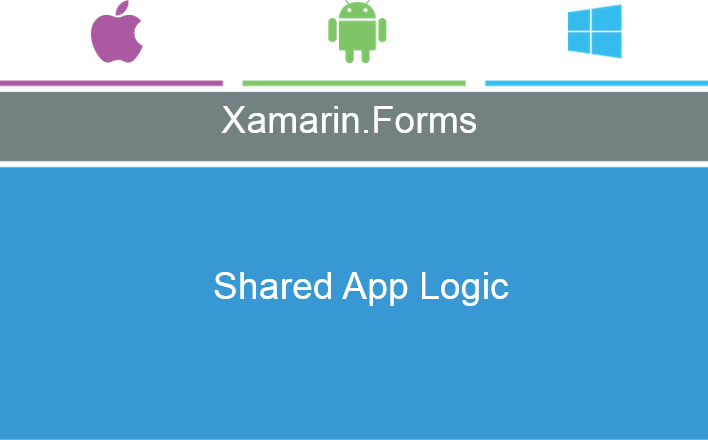
\includegraphics[width=1\textwidth]{images/code-sharing2.png}
		\caption{Xamarin.Forms Architektur (Quelle: https://blog.goyello.com/)}
		\label{fig:xamarinarchitectur}
	\end{figure}

	Abbildung \ref{fig:xamarinarchitectur} zeigt wie die Xamarin.Forms Architektur aussieht. Dabei werden die Nativen Bibliotheken von Android \textit{Android SDK}, iOS \textit{iOS UIKit} und Windows Phone bzw. Windows Mobile \textit{UWP SDK} eingebunden. Das Einbinden dieser Bibliotheken stellt dem Framework eine Vielzahl an UI Elementen zur Darstellung von Inhalten zur Verfügung. In der derzeitigen Version von Xamarin.Forms sind es 17 unterschiedliche Elemente.

	Jedoch ist zu beachten, dass der in Abbildung \ref{fig:xamarinarchitectur} in grau dargestellte Balken den Shared UI Code repräsentiert. Auf diesem aufbauend muss mit ungefähr 20\% Zielplattform spezifischen UI Design gerechnet werden \cite{book:Xamarin-Mobile-Application-Development}. Näheres dazu wird in den folgenden Abschnitten \ref{sec:xamarinformsmvvm} sowie \ref{chap:xamarinformsdevelopment} genauer erläutert.

	Wie Xamarin.Forms das rendern eines UI Elements durchführt ist in Abbildung \ref{fig:xamarinaformsrender} zu erkennen.

	\begin{figure}[h!]
		\centering
		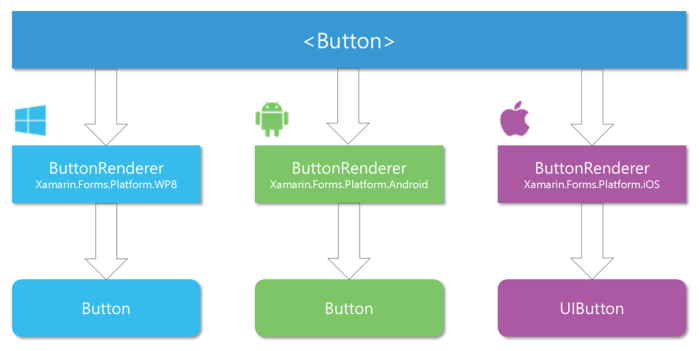
\includegraphics[width=0.9\textwidth]{images/xamarinforms-button-rendering.png}
		\caption[Wie Xamarin UI Elemente rendert]{Wie Xamarin UI Elemente rendert\\\hspace{\textwidth}(Quelle: igorelikblog.wordpress.com/2016/07/08/xamarin-form-memory-management)}
		\label{fig:xamarinaformsrender}
	\end{figure}

	Das Element \textbf{$<$Button$>$} wird im Layout File welches in XAML (Extensible Application Markup Language) geschrieben wurde, eingebaut. Wird der Code nun kompiliert ist der \textit{ButtonRenderer} jener Plattformspezifische renderer der, dass Xamarin.Forms UI Element in Nativen Code umsetzt. Der \textbf{$<$Button$>$} unter Xamarin.Forms wird dadurch in einen \textbf{UIButton} für iOS oder einen \textbf{Android.Button} für Android übersetzt. Dieses rendern macht Xamarin.Form einzigartig, da im Vergleich mit anderen Cross-platform Technologien das Design für die Zielplattformen meist mittels HTML oder CSS vorgenommen werden muss, um die UI Elemente in Native Design Elemente zu transformieren \cite{book:Xamarin-Mobile-Application-Development}.

	\textbf{Rendering} ist der Arbeitsschritt einer Bilderstellung aus Objekten die, wie im Beispiel des Xamarin.Forms Frameworks, aus grafischen Objekten bestehen, welche in XAML definiert wurden\footnote{https://www.itwissen.info/Rendering-rendering.html}.

	\textbf{XAML} ist die Beschreibungssprache die Xamarin verwendet um die grafische Gestaltung des UI zu ermöglichen. Da XAML nur eine Beschreibungssprache ist kann es keinen Code enthalten. Alle Event Handler, wie zum Beispiel das Klicken eines Button, müssen in einem Code File definiert werden.
	test

	\newpage
	Eine Standard XAML Datei ist in Abbildung \ref{fig:xamarinaformxamlpreview} dargestellt. Die Deklarationen in Zeile zwei bis drei definieren das der Namespace von Microsoft verwendet werden soll. In Zeile fünf wir ein Präfix für einen lokalen Namespace definiert um Zuweisungen im XAML File mit dem Code Behind File zu ermöglichen. Wird eine XAML Datei der PCL Klasse hinzugefügt, erzeugt die IDE neben der Layout Datei zusätzlich eine Code behind Datei. Diese ist in Abbildung \ref{fig:xamarinaformxamlpreview} als zweiter Tab zu erkennen. Über die Klasse \textit{MCKBPage.xaml.cs} wird das verhalten der App implementiert. Die Referenzierung erfolgt über die Namespace Deklarationen im XAML File.

	\begin{figure}[h!]
		\centering
		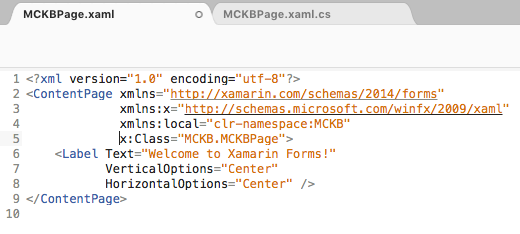
\includegraphics[width=1\textwidth]{images/XAML-preview.png}
		\caption[Aufbau einer XAML Datei für Xamarin.Forms]{Aufbau einer XAML Datei für Xamarin.Forms}
		\label{fig:xamarinaformxamlpreview}
	\end{figure}
	Für die Entwicklung der CP App wird Visual Studio for Mac verwendet, weil somit eine iOS Anwendung einfacher getestet werden kann. Man kann eine iOS App auch mit Windows erstellen, allerdings benötigt man dazu einen Mac im gleichen WLAN Netzwerk damit der Compiler die App erzeugen und ausführen kann.

	\newpage
	\textbf{PCL} steht für Portable Class Library und ist jene Klasse in welcher sich der gemeinsame Code für die Cross-platform App befindet.
	
	\begin{figure}[h!]
		\centering
		\begin{minipage}{.4\textwidth}
			\centering
			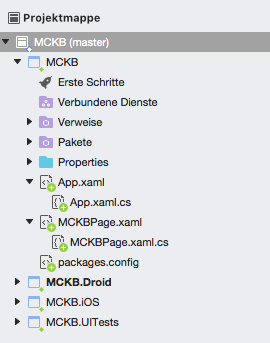
\includegraphics[width=.9\textwidth]{images/project-structure.png}
        	\label{fig:xamarinformprojectstructure}
			\caption[Projekt Struktur einer CP App]{\\\hspace{\textwidth}Projekt Struktur einer CP App}
		\end{minipage}
		\begin{minipage}{.5\textwidth}
			In Abbildung 2.4 sind alle relevanten Klassen aufgelistet die für eine Cross-platform Applikation benötigt werden. Die \textbf{PCL} Klasse ist im Ordner \textit{MCKB} implementiert. Die weiteren Ordner beginnend mit \textit{MCKB.} gefolgt von \textit{Droid} oder \textit{iOS} können dafür verwendet werden gezielt Plattformspezifischen Code zu implementieren welcher nicht von beiden Zielbetriebssystemen verwendet wird. 
        	Weiters ist das XAML File aus Abbildung \ref{fig:xamarinaformxamlpreview} mit dessen Code Behind File zu erkennen. Die Ordner, \textit{Verweise} werden benötigt damit der Compiler die korrekte Zuordnung zum Zielbetriebssystem durchführen kann. Der Ordner \textit{Pakete} ermöglicht es Pakete des \textbf{NuGET} Paket Managers einzubinden. Ein solches Paket kann beispielsweise eine MySQL Anbindung an einen Server sein.
        \end{minipage}
	\end{figure}
	Die in Abbildung \ref{fig:xamarinformprojectstructure} wird im Laufe der Entwicklung um einige XAML und Code Behind Files wachsen. Der Prozess der Programmierung ist in Abschnitt \ref{chap:xamarinformsdevelopment} festgehalten.
	\newpage

\section{Entwicklung unter Xamarin.Forms}
\label{sec:xamarinformsdevelopement}

	Wie schon in Abschnitt \ref{chap:xamarin} eingangs kurz angeschnitten wurden die Unterschiede der Kompilierung von Xamarin aufgezeigt. Als Entwickler kann man in C\# auf die schon bekannten .NET Klassen, aufgrund von Mono zugreifen und die Applikationslogik implementieren. Ist die App für den ersten Testlauf bereit, wählt man in der Projekt Struktur die Zielplattform aus und markiert diese als Start Projekt. In Abbildung \ref{fig:xamarinformprojectstructure} ist dies zum Beispiel \textit{MCKB.Droid}, da dieser Ordner durch eine Dicke Schrift hervorgehoben wurde.

	Der Prozess der Kompilierung ist in Abbildung \ref{fig:xamarinanativeandroidcompile} zu erkennen.
	\begin{figure}[h!]
		\centering
		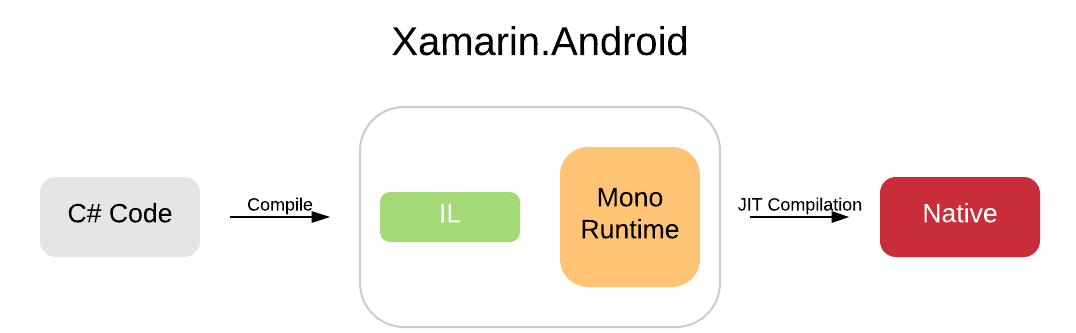
\includegraphics[width=1\textwidth]{images/Xamarin-Android.png}
		\caption{Wie Xamarin.Android kompiliert wird}
		\label{fig:xamarinanativeandroidcompile}
	\end{figure}

	Der C\# Code wird in die Intermediate Language (IL) umgesetzt und in die Mono Runtime geladen. Anschließend übernimmt der Just-In-Time (JIT) Compiler die Übersetzung in Nativen Code der anschließend auf dem Zielbetriebssystem ausgeführt wird. Dieser Prozess läuft im Xamarin Frameworks automatisch ab sobald die Applikation erstellt und auf das Virtuelle oder Hardware Gerät geladen werden soll.

	Wählt man in Abbildung \ref{fig:xamarinformprojectstructure} iOS als Startprojekt, \textit{MCKB.iOS} ist dann Dick hervorgehoben, so sieht der Erstellungsprozess differenzierter aus, da Apple eine JIT Kompilierung nicht unterstützt. Betrachtet man Abbildung \ref{fig:xamarinanativeioscompile} genauer erklärt es warum man einen Apple Computer für die Erstellung einer iOS oder MacOS Anwendung benötigt.
	\begin{figure}[h!]
		\centering
		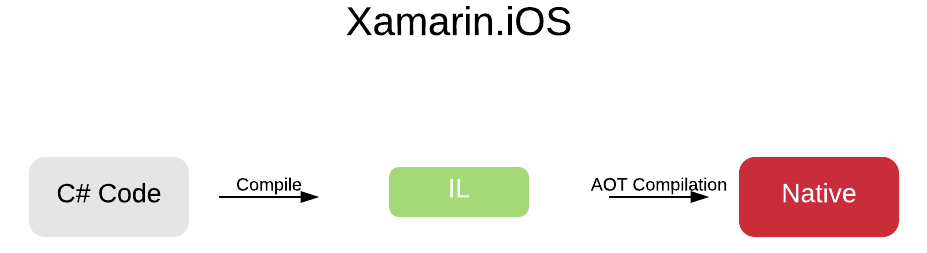
\includegraphics[width=1\textwidth]{images/Xamarin-iOS.png}
		\caption{Wie Xamarin.iOS kompiliert wird}
		\label{fig:xamarinanativeioscompile}
	\end{figure}

	Für die Erstellung der iOS App wird gleich wie bei einer Android App der C\# Code in die IL kompiliert. Da nun keine Mono Runtime zur Verfügung steht wird ein Apple Compiler benötigt. Dieser Compiler ist der Ahead-of-Time (AOT) Compiler der nun die Übersetzung in Nativen Code übernimmt.

	Xamarin.Forms stellt eine höhere Abstraktions Ebene für die Entwicklung einer Applikation dar. Der Kompilierungsprozess lässt sich folgendermaßen darstellen.
	\begin{figure}[h!]
		\centering
		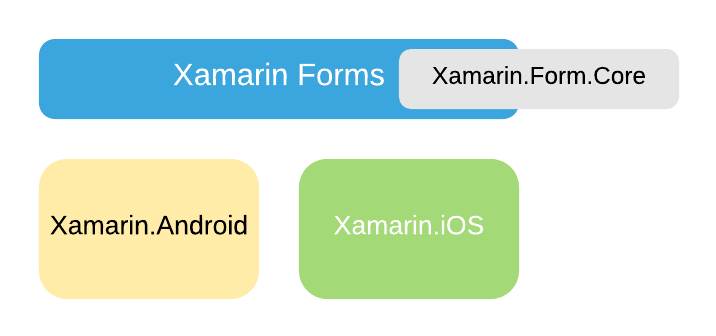
\includegraphics[width=1\textwidth]{images/Xamarin-Forms.png}
		\caption{Xamarin.Forms Architektur}
		\label{fig:xamarinformsarchitecture}
	\end{figure}

	Abbildung \ref{fig:xamarinformsarchitecture} beschreibt was durch Xamarin.Forms erzielt werden soll. Es baut auf den Bibliotheken für die Übersetzung in Nativen Android und iOS Code auf und ist das fehlende Bindeglied für den Prozess in Abbildung \ref{fig:xamarinaformsrender} (Rendering eines Button von Xamarin.Forms). Jener Part der für die Übersetzung des Codes zuständig ist, ist die \textit{Xamarin.Forms.Core} Bibliothek. Die in dem XAML File festgelegten UI Elemente der PCL Klasse sind Teil dieser \textit{Xamarin.Forms.Core} Bibliothek. Der Compiler übersetzt nun für die UI ELemente für Android, siehe Abbildung \ref{fig:xamarinanativeandroidcompile} und iOS, siehe Abbildung \ref{fig:xamarinanativeioscompile}, damit das Zielplattform spezifische Design dargestellt wird.
	\newpage

\subsection{Model View View Model - Design Pattern}
\label{sec:xamarinformsmvvm}

\newpage
\subsection{Projekterstellung mit Visual Studio for Mac}
\label{sec:xamarincreateproject}

	Für die Entwicklung der Cross-Platform Applikation wird \textbf{Visual Studio for Mac} verwendet im sowohl eine Android als auch iOS Version der Applikation entwickeln zu können. Die Projekterstellung unter Windows mit \textbf{Visual Studio 2015} oder \textbf{2017} verläuft analog im gleichen Schema.

	Zu Beginn wird eine Standard Xamarin.Forms Applikation erstellt. Hierbei muss entschieden werden wie der Cross-Platform Code geteilt werden soll:

	\begin{figure}[h!]
		\centering
		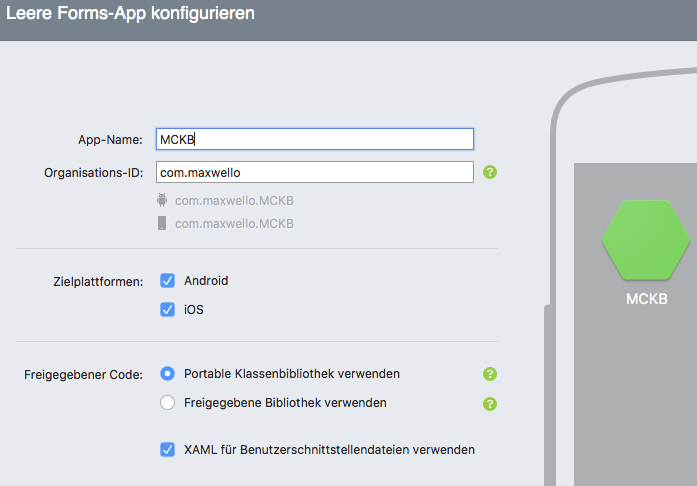
\includegraphics[width=1\textwidth]{images/Project-Setup-one.png}
		\caption{Erstellung der Xamarin.Forms App - MCKB}
		\label{fig:xamarinprojectstart}
	\end{figure}

	In Abbildung \ref{fig:xamarinprojectstart} ist zu erkennen das schon bei der Erstellung der Applikation festgelegt werden muss auf welche Art und Weise der \textit{Shared Code}, der CP-App implementiert werden soll.

	In Abbildung \ref{fig:xamarinsharedcode} ist zu erkennen wie sich \textbf{Portable Class Library} von \textbf{Shared Library} unterscheiden. Wird PCL für den freigegeben Code verwendet, siehe Abbildung \ref{fig:xamarinsharedcode} links, so erstellt die IDE alle notwendigen Verweise und verlinkt diese. Anders ist dies bei einem Shared Library (SL) Projekt, bei welchem der Entwickler selbst die notwendigen Verweise zu weiteren dependencies einbinden muss.

	\newpage
	\begin{figure}[h!]
		\centering
		\begin{subfigure}
			\centering
			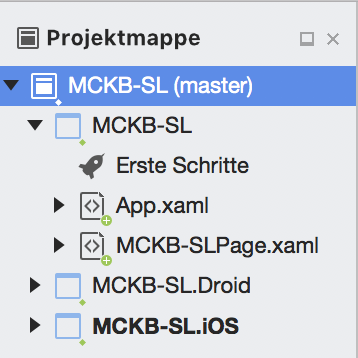
\includegraphics[width=.3\textwidth]{images/xamarin-shared-library.png}
		\end{subfigure}
		\begin{subfigure}
			\centering
			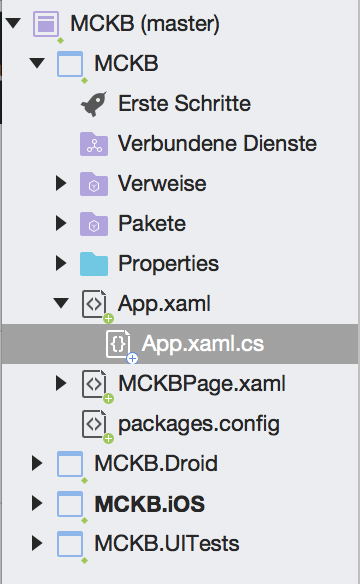
\includegraphics[width=.3\textwidth]{images/xamarin-portable-class.png}
		\end{subfigure}
		\caption{Unterschied Shared Code - Xamarin.Forms App - MCKB}
		\label{fig:xamarinsharedcode}
	\end{figure}

	Der Unterschied bei der Festlegung auf welche Art und Weise der freigegebene Code für die Applikation verwaltete werden soll muss von Beginn an definiert werden. Eine Änderung im Nachhinein ist nicht mehr möglich.

	\textbf{Eine Portable Klassenbibliothek (\textit{PCL})} erstellt wie schon erwähnt alle notwendigen Verweise für eine Android und iOS Cross-Plattform Applikation. Dabei spielen die folgenden Verweise eine wichtige Rolle:
	\begin{itemize}
		\setlength\itemsep{0em}
		\item \textit{Xamarin.Forms.Core} definiert eine allgemeine API (Application Programming Interface) für Klassen wi zum Beispiel Buttons, Labels, ListViews uvm.
		\item \textit{Xamarin.Forms.Platform} linkt die Plattform spezifischen Renderer von Android und iOS damit Elemente in der PCL Klasse in Plattform spezifischen Code übersetzt werden können.
		\item \textit{Xamarin.Forms.Xaml}
	\end{itemize}

	\textbf{Die Freigegeben Bibliothek (\textit{Shared Library})} 
























          % Background - Xamarin

%----------------------------------------------------------------
%
%  File    :  chapter3.tex
%
%  Authors :  Keith Andrews, IICM, TU Graz, Austria
%             Manuel Koschuch, FH Campus Wien, Austria
% 
%  Created :  22 Feb 96
% 
%  Changed :  30 Oct 2008
%  !TEX root = ./thesis.tex
%----------------------------------------------------------------


\chapter{Entwicklung der MCKB Applikation}
\label{chap:xamarinformsdevelopment}

Die im 4. Semester entwickelte \textit{STM32KB} APP welche Nativ in Adroid geschrieben wurde ist die Grundlage der \textit{MCKB} Cross-Platform APP. 

\section{Applikations Spezifizierung}
\label{sec:mckspecs}

\subsection{Funktionale Anforderungen}
\label{sec:mckbfunkcspecs}

\subsection{Nicht Funktionale Anforderungen}
\label{sec:mckbnonfuncspecs}

\section{Unterschiede zur Xamarin.Native Version}
\label{sec:mckbspecs}          % The App - MCKB

%----------------------------------------------------------------
%
%  File    :  chapter4.tex
%
%  Authors :  Keith Andrews, IICM, TU Graz, Austria
%             Manuel Koschuch, FH Campus Wien, Austria
% 
%  Created :  22 Feb 96
% 
%  Changed :  30 Oct 2008
%  !TEX root = ./thesis.tex
%----------------------------------------------------------------


\chapter{Ergebnisse}
\label{chap:xamarinformsresults}

	Im Zuge der Spezifizierung und Entwicklung mit Visual Studio for Mac \textit{früher Xamarin Studio} ist es zu einigen Hürden gekommen. Angefangen bei der Projekt Erstellung, da Xamarin.Native und Xamarin.Forms in regelmäßigen Abständen Updates für die IDE's veröffentlicht. Dabei ist es immer wieder dazu gekommen das die Entwicklungsumgebung keine der CP Applikationen erstellen konnte. Um dieses Problem zu umgehen dürfen nach der Projekterstellung die Paket Aktualisierungen nicht gemacht werden. Wird das Projekt mit einer Xamarin.Forms Version erstellt kann damit ohne Probleme gearbeitet werden. Ein Aktualisieren der Plugins und Pakete wird dann notwendig wenn man auf Funktionen einer neueren Xamarin.Forms Version zugreifen will.

	Somit musste die MCKB App mit Xamarin.Forms in der Version \textbf{2.5.0.121934} entwickelt werden. Wurde Xamarin.Forms auf, die zu diesem Zeitpunkt geschriebene Arbeit, Version \textbf{3.0.0.482510} aktualisiert so erhielt man bei Erstellung der iOS oder Android App, die in Abbildung dargestellte Fehlermeldung. Der Fehler konnte trotz einer VIelzahl an Workarounds und diverser Anpassungen an den Referenzen in den Verweisen des Projekt behoben werden. Ein Aktualisieren der Pakete und Plugins wurde deshalb vermieden.

	\begin{figure}[h!]
		\centering
		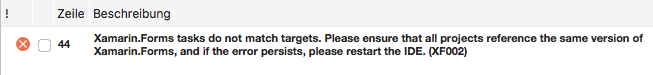
\includegraphics[width=1\textwidth]{images/Xamarin-Upgrade-Error.png}
		\caption{Fehlermeldung nach Aktualisierung aller Projektpakete}
		\label{fig:xamarinbuilderror}
	\end{figure}

	\newpage
	Der Einsatz von Webservices, siehe Abschnitt \ref{sec:mckbspecs}, ist einerseits auf die Deaktivierung des Xamarin Komponenten Store und andererseits auf die in Codeabschnitt \ref{lst:pluginerror} dargestellte Fehlermeldung bei hinzufügen des Plugins, \textbf{Xamarin.MySQL.Data.1.0.1} zurückzuführen.

	\begin{lstlisting}[caption={Fehlermeldung - Plugin Installation},label={lst:pluginerror},captionpos=b,style=SQL-Michalstyle]
Install failed. Rolling back...
Package 'Xamarin.MySql.Data.1.0.1' does not exist in project 'MCKB'
Package 'Xamarin.MySql.Data.1.0.1' does not exist in folder 
'/Users/maximilianpessl/Projects/MCKB/packages'
Executing nuget actions took 46,83 ms
Could not install package 'Xamarin.MySql.Data 1.0.1'. 
You are trying to install this package into a project that targets 
'.NETPortable,Version=v4.5,Profile=Profile7', 
but the package does not contain any assembly references or 
content files that are compatible with that framework. 
For more information, contact the package author.
	\end{lstlisting}

	Anpassungen an dem Projekt (MCKB PCL), zum Beispiel ändern der PCL Einstellungen welche in Zeile acht in Codeabschnitt \ref{lst:pluginerror} dargestellt sind, haben diese Fehlermeldung nicht beheben können, wodurch auf \textit{REST} als Webservice API zurückgegriffen werden musste. Das Plugin konnte den Projekten \textit{MCKB.Droid} und \textit{MCKB.iOS} hinzugefügt werden, jedoch bedeutete dies, dass die Client (Smartphone App) Server Kommunikation in beiden Projektordnern implementiert werden musste.

	Zur Messung der Kommunikationszeit zwischen dem Senden eines \textit{GET Request} und Empfangen einer \textit{Response} wurden vor dem Senden bzw. nach Empfangen die Systemzeit erhoben und in folgender Tabelle\ref{tab:clsvcom}\footnote{Xam.Forms.x - Xamarin.Forms.x App \\Xam.Nat.x - Xamarin.Native.x App \\Nat.Droid - Native Android\\ S - Send // R - Receive} festgehalten. Der dafür notwendige Code steht in Abschnitt \ref{chap:app} Codeabschnitt \ref{lst:measurecom} zur Verfügung.

	\begin{table}[h!]
		\centering
		\begin{tabular}{l|l|l|l|l|l|}
			\cline{2-6}
			                        & Xam.Forms.iOS    & Xam.Forms.Droid  & Xam.Nat.Droid& Xam.Nat.iOS  & Nat.Droid    \\ \hline
			\multicolumn{1}{|l|}{S} & 14:18:19.3465230 & 14:33:58.4397800 & 22:58:54.588 & 22:48:32.136 & 22:38:21.135 \\ \hline
			\multicolumn{1}{|l|}{R} & 14:18:19.8951310 & 14:34:01.3333110 & 22:58:54.717 & 22:48:32.260 & 22:38:37.775 \\ \hline
			\multicolumn{1}{|l|}{S} & 15:08:08.6368570 & 15:06:01.3397350 & - & - & - \\ \hline
			\multicolumn{1}{|l|}{R} & 15:08:09.3322090 & 15:06:03.1629580 & - & - & - \\ \hline
			\multicolumn{1}{|l|}{S} & 15:08:59.3353410 & 15:09:50.1086710 & - & - & - \\ \hline
			\multicolumn{1}{|l|}{R} & 15:08:59.8671340 & 15:09:51.9077950 & - & - & - \\ \hline
		\end{tabular}
		\label{tab:clsvcom}
		\caption{Ergebnisse der Kommunikationszeit über Webservice - Gegenüberstellung mit früheren Ergebnissen\cite{Maximilian2017} - Smartphone Simulatoren/Emulatoren}
	\end{table}
	
	
	\newpage
	Leider war es nicht möglich eine Messung für ein iOS und Android Smartphone durchzuführen, da es nicht möglich war die MCKB App auf einem iOS Gerät zu installieren. In Tabelle \ref{tab:clsvcomhard} sind daher nur die Ergebnisse der Android Version auf einem Alcatel Smartphone festgehalten.

	\begin{table}[h!]
		\centering
		\begin{tabular}{l|l|l|l|l|l|}
			\cline{2-6}
			                        & Xam.Forms.iOS    & Xam.Forms.Droid  & Xam.Nat.Droid& Xam.Nat.iOS  & Nat.Droid    \\ \hline
			\multicolumn{1}{|l|}{S} & 	  -			 & 14:32:04.8747300 & 		-	   & 	  -		  &  \\ \hline
			\multicolumn{1}{|l|}{R} & 	  -			 & 14:32:08.8170480 & 		-	   & 	  -		  &  \\ \hline
			\multicolumn{1}{|l|}{S} & 	  -			 & 15:12:15.8343150 & 		-	   & 	  -		  &  \\ \hline
			\multicolumn{1}{|l|}{R} & 	  -			 & 15:12:19.6612780 & 		-	   & 	  -		  &  \\ \hline
			\multicolumn{1}{|l|}{S} & 	  -			 & 15:13:21.6869140 & 		-	   & 	  -		  &  \\ \hline
			\multicolumn{1}{|l|}{R} & 	  -			 & 15:13:25.2504780 & 		-	   & 	  -		  &  \\ \hline
		\end{tabular}
		\label{tab:clsvcomhard}
		\caption{Ergebnisse der Kommunikationszeit über Webservice - Gegenüberstellung mit früheren Ergebnissen\cite{Maximilian2017} - Smartphone Hardware}
	\end{table}

	Eine Gegenüberstellung der Android App (STM32KB) mit dessen CP Versionen (STM32CP \& MCKB) war aufgrund der Änderungen seitens Microsoft nicht möglich. Da der Komponenten Store entfernt wurde kann die STM32CP App nicht mehr erstellt werden.

	Jedoch ist in beiden Tabellen erkennbar das es signifikante Unterschiede zwischen den CP Versionen der STM32KB App gab. Die Ladezeiten der Xamarin.Native App ist um einiges geringer als die der Xamarin.Forms Applikationen, wobei die Xamarin.Forms.iOS annähernd gleich schnell die Daten aus der Datenbank in die Applikation geladen hat.

	Die deutlich unterschiedlichen Ladezeiten für die Xamarin.Forms.Droid App könnten dadurch erklärt werden das ein Android Emulator nur die notwendigsten Systemprozesse im Hintergrund laufen lässt, während ein echtes Smartphone deutlich ausgelasteter ist.

	Bezüglich des Designs und der Programmierung der MCKB App bietet Xamarin.Forms eindeutig einen Zeitgewinn. Der Umstand bis zu 80 oder 90\% des Designs und der Geschäftslogik in dem PCL Projekt umzusetzen ist, sofern aufgrund der Spezifizierung möglich, genau das was CP-Developing so attraktiv macht. Allerdings gibt es eine Einschränkung bezüglich der MCKB.Droid App. In der Xamarin.Native Version gab es in der \textit{MainActivity} mehrere \textit{Fragments} um das Layout schnell wechseln zu können. Die Implementierung von Fragment ist im PCL Projekt nicht möglich. Weiters impliziert der Name Xamarin.Forms das es sich dabei um ein UI Framework mit klaren entscheidungsbasierten oder formularbasierten Abläufen in der App handelt. Erfordert eine CP App viele komplexe UI ELemente so empfiehlt es sich diese mit Xamarin.Native zu entwickeln. Da die MCKB App keine komplexen UI Elemente benötigt eignete sich Xamarin.Forms als Framework sehr gut.

	Das Design wird, wie Eingans erwähnt im PCL Projekt für iOS und Android gemeinsam in den jeweiligen \textit{XAML} Files erstellt. Zwar stellt Visual Studio for Mac eine Vorschau, für das Editieren von Design Files zur Verfügung, jedoch gab es hier immer wieder Probleme mit dem Rendern der UI Elemente. In Abbildung \ref{fig:mckbAppregister}\footnote{Der XAML Code befindet sich im Abschnitt \ref{chap:app} Codeabschnitt \ref{lst:mckbcodereg}} ist zur erkennen das man durch hinzufügen des \textit{BackgroundColor} Parameters die Ränder des Layout Elements darstellen kann um so die Grenzen eines \textit{StackLayout}, wie es die Page in Abbildung \ref{fig:mckbAppregister} verwendet, darzustellen.

	\begin{figure}[h!]
		\centering
		\begin{subfigure}
			\centering
			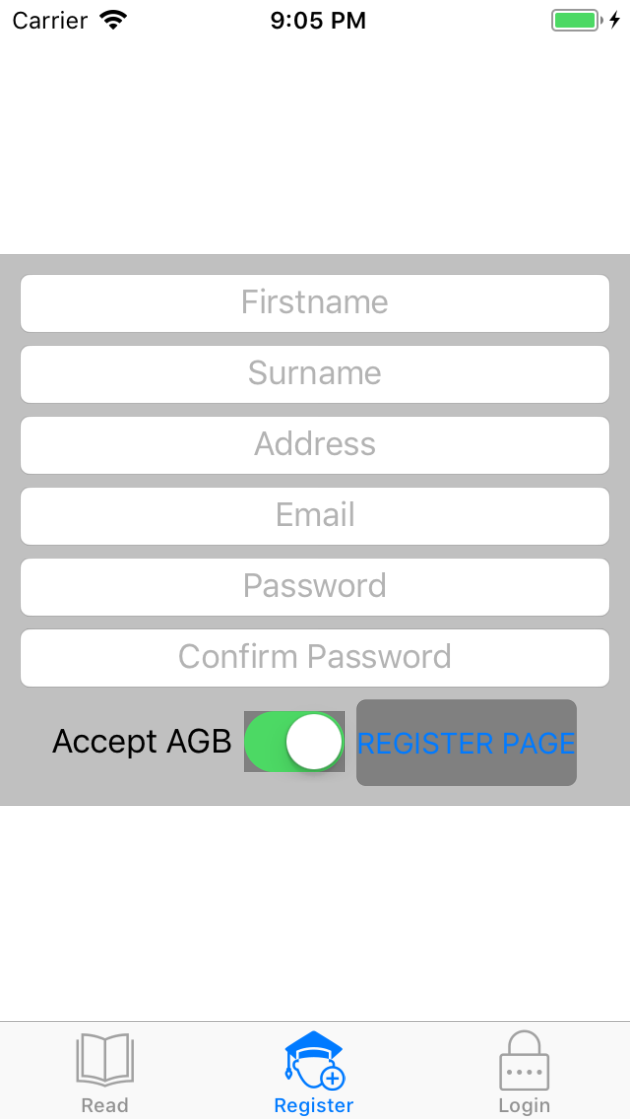
\includegraphics[width=.4\textwidth]{images/MCKB-iOS-Register-edit.png}
		\end{subfigure}
		\begin{subfigure}
			\centering
			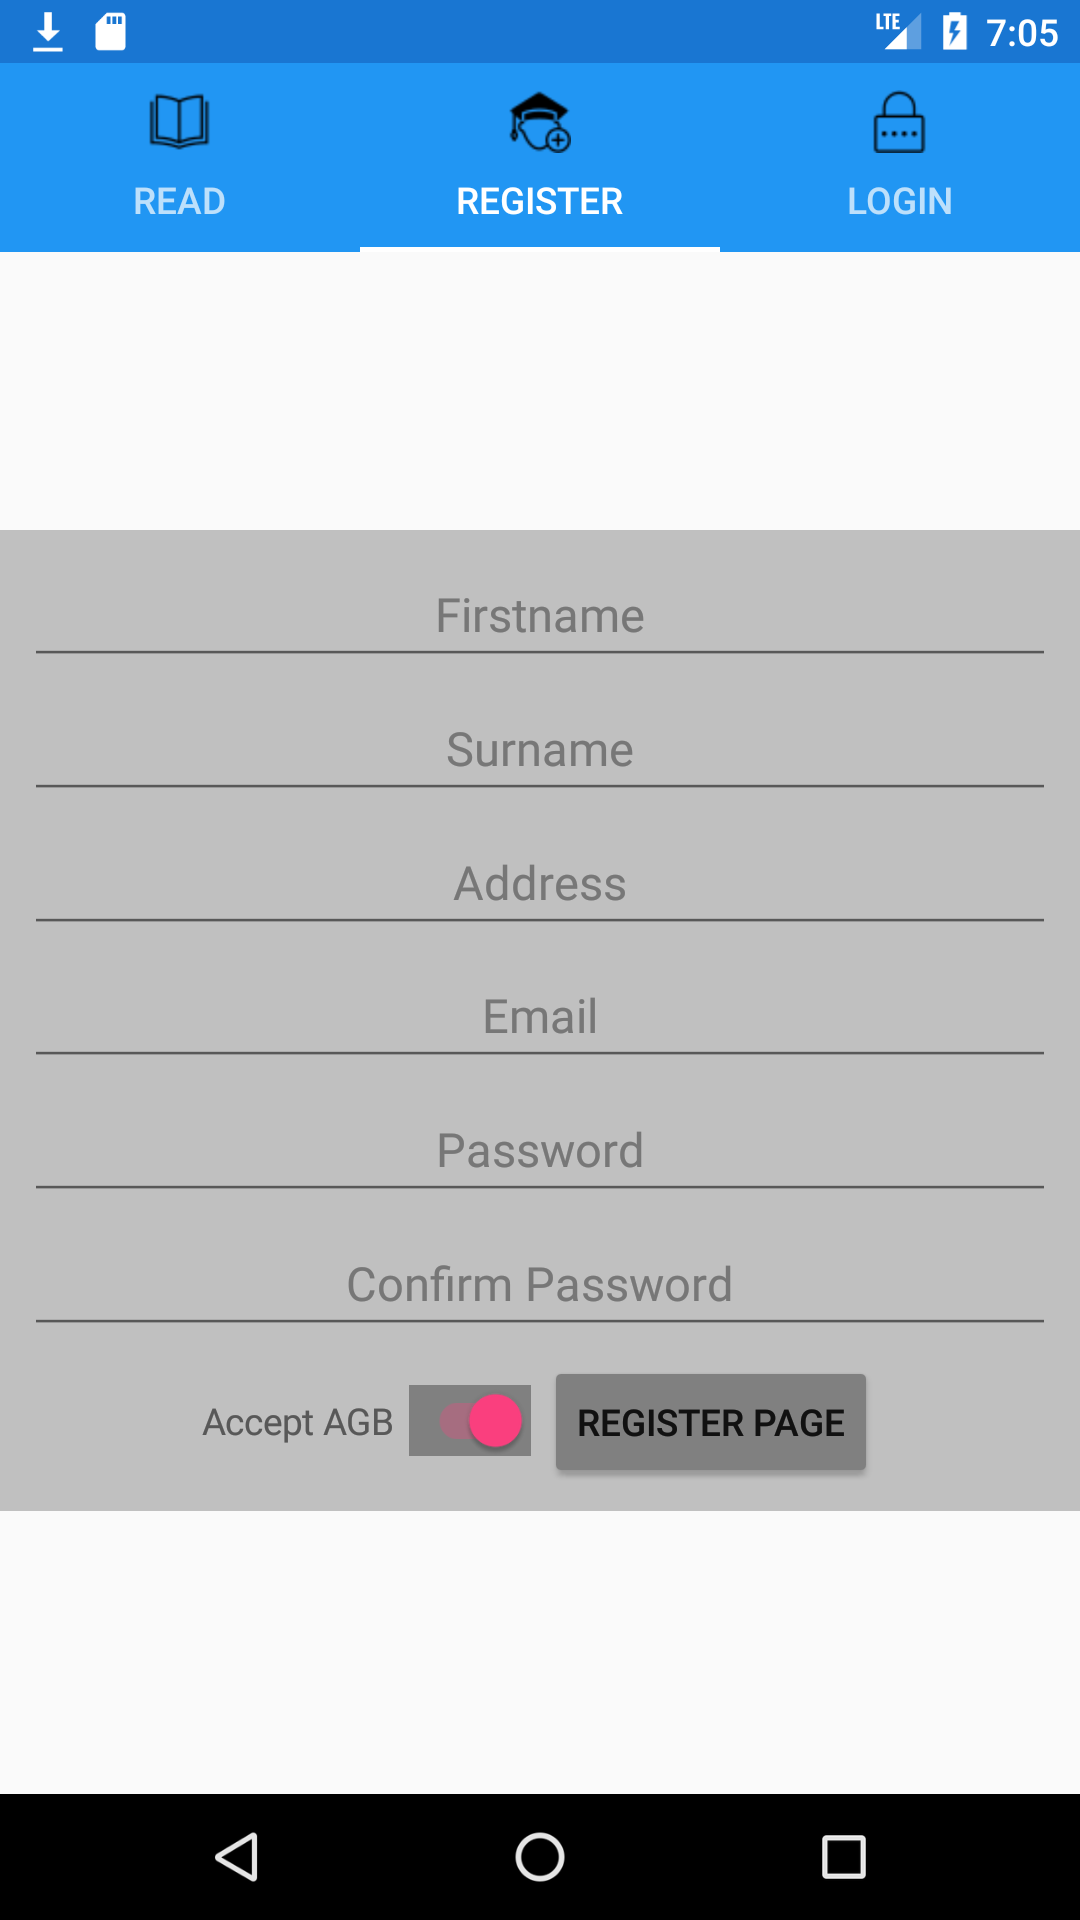
\includegraphics[width=.4\textwidth]{images/MCKB-Droid-Register-edit.png}
		\end{subfigure}
		\caption{Darstellen von Layout Grenzen}
		\label{fig:mckbAppregister}
	\end{figure}

	Selbiger Ansatz zur Abschätzung der Größe der UI Elemente wurde für die Login Page verwendet.

	In Kapitel \ref{chap:xamarinformsdevelopment} Abschnitt \ref{sec:mckspecs} ist die Spezifizierung für den \textit{UseCase - Artikel lesen} so definiert das durch eine Kategorie an Mikrocontroller die Artikel einer Kategorie durch Auswahl eines Dropdown angezeigt werden. Im Zuge der Programmierung wurde dies angepasst, ersichtlich in Abbildung \ref{fig:mckbApp}, da mit einer Liste an Kategorien die wiederum eine Liste an Artikeln enthält ein moderneres Design entworfen werden konnte.

	Das endgültige Design der MCKB Applikation ist in Kapitel \ref{chap:app} in Abbildung \ref{fig:mckbAppfinal} dargestellt. Der Code für dieses Design ist in Codeabschnitt \ref{lst:mckbdesigncode} zu finden. Plattformspezifische Design Parameter sind durch den \textbf{tag} \textit{$<$OnPlatform$><$/OnPlatform$>$} definiert. 




          % Results

%----------------------------------------------------------------
%
%  File    :  chapter5.tex
%
%  Authors :  Keith Andrews, IICM, TU Graz, Austria
%             Manuel Koschuch, FH Campus Wien, Austria
% 
%  Created :  22 Feb 96
% 
%  Changed :  30 Oct 2008
%  !TEX root = ./thesis.tex
%----------------------------------------------------------------


\chapter{Fazit}
\label{chap:xamarinformsconclusion}

	Für die Programmierung von Software auf den Vollen Funktionsumfang eines Frameworks zurückgreifen zu können ermöglicht es Probleme gezielt zu lösen. Dabei leuchtet es ein, dass ein Framework wie beispielsweise Xamarin.Forms nur einen Teil des Funktionsumfanges der Zielplattform zur Verfügung stellt. Kreativität und Erfahrung in der Software/Applikationsentwicklung spielen hierbei ein Große Rolle das Framework so zu verwenden um die Software Anforderungen umzusetzen.

	Analyse und Design waren vor Beginn und während der Entwicklung der MCKB CP App ständig präsent und haben direkten Einfluss eingenommen. Wurde zum Beispiel das iOS Projekt exakt der Vorgaben in dem Design File angezeigt, mussten immer wieder kleine Änderungen an der Android Version vorgenommen werden. Jedoch musste dabei kein Android spezifischer Code geschrieben werden, sondern durch plattformspezifische Parametrierung jene Anpassung vorgenommen werden um ein ähnlich Strukturiertes Design wie in der iOS Version zu erzielen. Anfängliche Stolpersteine die nach wenigen Zeilen Code aufgetreten sind konnten sowohl durch Recherche zu den Besonderheiten von Xamarin.Forms als auch Kreativität, aus dem Weg geräumt werden.

	Der Umstand das Xamarin.Forms den großen Vorteil hat wenig Code doppelt oder dreifach zu schreiben steht dessen Eingeschränkten Funktionsumfang für plattformspezifische Funktionen gegenüber. Ist man es gewohnt Probleme die eventuell nur Android betreffen in dessen Projekt statt der PCL zu beheben so ist dies zwar möglich, kann im Verlauf jedoch zu ungewollten Nebeneffekten im weiteren Verlauf der Programmierung führen. Speziell bei der Entwicklung der MCKB App kam es immer wieder vor das ein spezifisches Problem zuerst im Projekt der Zielplattform behoben werden kann, jedoch beim Aufkommen eines ähnlichen Problems das Design zur Funktion die jenes Problem lösen soll überdacht werden musste.

	Ein direkter Vergleich der Funktionen der Android App mit der CP App zeigt, dass das immerwährende überdenken des Design dazu geführt hat das die Applikation laufend evaluiert worden ist. Und dabei sogar für zwei Zielplattformen zur gleichen Zeit. Jedoch spielte die erste CP App (STM32CP) eine essenzielle Rolle, weil bei der Entwicklung jener App viele Erfahrungen gesammelt werden konnten.

	Bla Bla
          % Conclusion

\appendix

%----------------------------------------------------------------
%
%  File    :  appendix.tex
%
%  Authors :  Keith Andrews, IICM, TU Graz, Austria
%             Manuel Koschuch, FH Campus Wien, Austria
% 
%  Created :  22 Feb 96
% 
%  Changed :  30 Oct 2008
%  !TEX root = ./thesis.tex
%----------------------------------------------------------------
\renewcommand*{\lstlistlistingname}{Codeverzeichnis}
\chapter{Anhang/Ergänzende Information}
\label{chap:app}
	% \begin{figure}[h!]
	% 	\centering
	% 	\begin{subfigure}
	% 		\centering
	% 		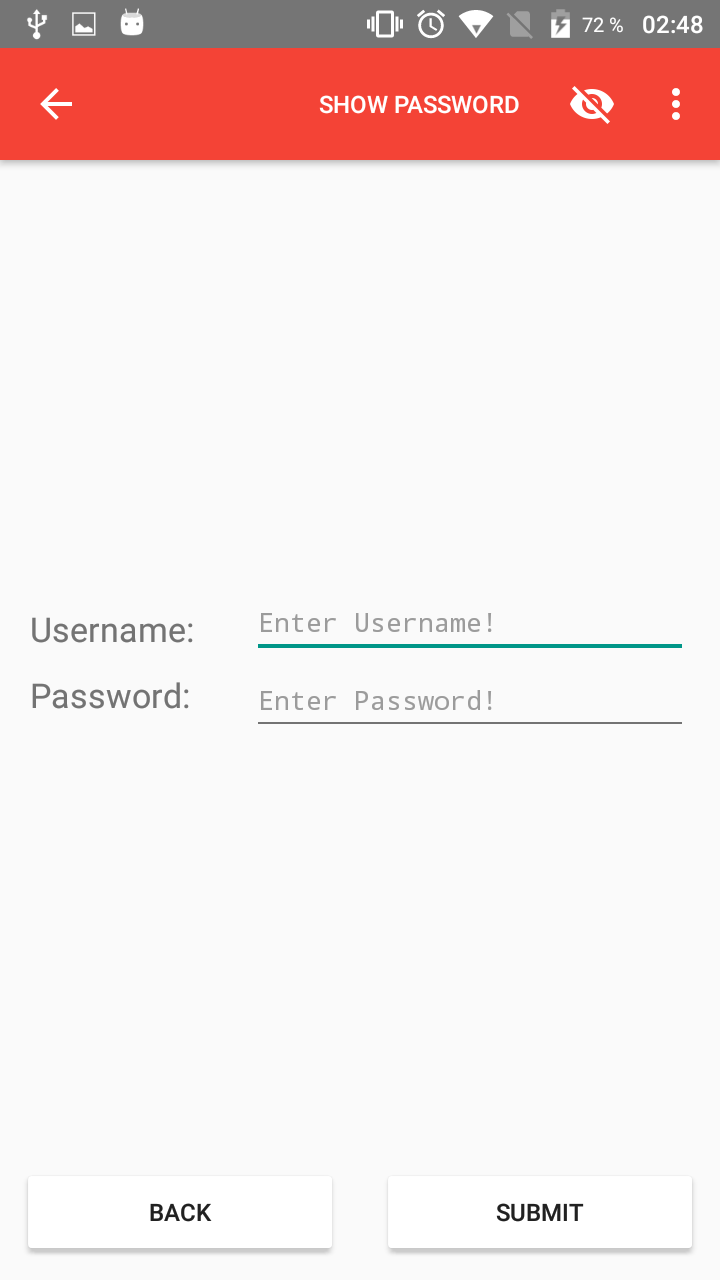
\includegraphics[width=.3\textwidth]{images/stm32kb-loginscreen.png}
	% 	\end{subfigure}
	% 	\label{fig:nope}
	% \end{figure}
	\begin{figure}[h!]
		\centering
		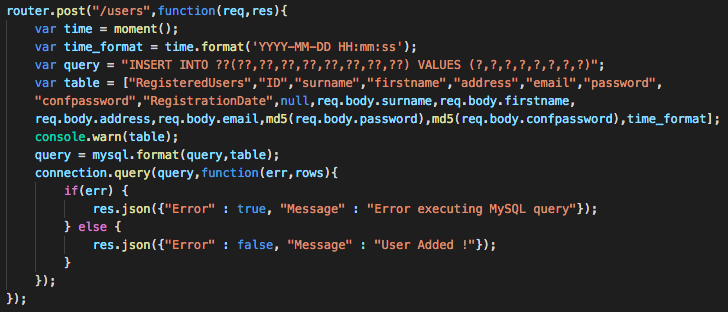
\includegraphics[width=1\textwidth]{images/restfull-server-code.png}
		\caption{RESTful - Server code - User Anlegen}
		\label{fig:serversidecode}
	\end{figure}

	\begin{lstlisting}[caption={Messung der Kommunikationszeit - MCKB PCL},label={lst:measurecom},captionpos=b,style=csharp]
protected override async void OnAppearing(){
    // Measing how long a request takes - START
    DateTime Jan1970 = new DateTime(1970, 1, 1, 0, 0, 0, DateTimeKind.Utc);
    TimeSpan javaSpan = DateTime.UtcNow - Jan1970;
    var time = DateTime.Now.Millisecond.ToString();
    var time3 = DateTime.UtcNow.ToString();
    System.Diagnostics.Debug.WriteLine(javaSpan + " Sending Request");
    var content = await _client.GetStringAsync(Url);
    var articles = JsonConvert.DeserializeObject<List<Article>>(content);
    DateTime Jan19702 = new DateTime(1970, 1, 1, 0, 0, 0, DateTimeKind.Utc);
    TimeSpan javaSpan2 = DateTime.UtcNow - Jan19702;
    var time2 = DateTime.Now.Millisecond.ToString();
    var time4 = DateTime.UtcNow.ToString();
    System.Diagnostics.Debug.WriteLine(javaSpan2 + " Received Request");
    // Measing how long a request takes - END
...}
	\end{lstlisting}

	\begin{lstlisting}[caption={MCKB Code-behind - Webservice Call},label={lst:mckbcoderegweb},captionpos=b,style=csharp]
...
namespace MCKB{
    public partial class MainPage : TabbedPage {
        private const string Url = "http://m4xwe11o.ddns.net:8000/api/articles";
        private HttpClient _client = new HttpClient();
        private ObservableCollection<Article> _articles;
		...
        protected override async void OnAppearing(){
        	...
            var content = await _client.GetStringAsync(Url);
            var articles = JsonConvert.DeserializeObject<List<Article>>(content);
			...
            _articles = new ObservableCollection<Article>(articles);
            ...
        }
    }
}

	\end{lstlisting}

	\begin{lstlisting}[caption={MCKB XAML Code für Registrierung},label={lst:mckbcodereg},captionpos=b,style=XML-Own]
<!--Tabbed Page two is for the registration of an user -->
<ContentPage Title="Register" Icon="icons8studentregistrationfilled.png">
    <ContentPage.Padding>
        <OnPlatform x:TypeArguments="Thickness" iOS="0,20,0,0" Android="0,0,0,0"></OnPlatform>
    </ContentPage.Padding>
    <StackLayout HorizontalOptions="FillAndExpand" VerticalOptions="Center" BackgroundColor="Silver" Padding="10,10,10,10">
        <Entry HorizontalTextAlignment="Center" Placeholder="Firstname"/>
        <Entry HorizontalTextAlignment="Center" Placeholder="Surname"/>
        <Entry HorizontalTextAlignment="Center" Placeholder="Address"/>
        <Entry HorizontalTextAlignment="Center" Placeholder="Email" Keyboard="Email"/>
        <Entry HorizontalTextAlignment="Center" Placeholder="Password" IsPassword="true"/>
        <Entry HorizontalTextAlignment="Center" Placeholder="Confirm Password" IsPassword="true"/>
        <StackLayout HorizontalOptions="Center" VerticalOptions="CenterAndExpand">
            <StackLayout Orientation="Horizontal" Padding="0,0,0,0">
                <Label Text="Accept AGB" VerticalOptions="Center"/>
                <Switch IsToggled="false" x:Name="accept" BackgroundColor="Gray" VerticalOptions="Center"/>
                <Button Text="REGISTER PAGE" IsEnabled="{Binding Source={x:Reference accept}, Path=IsToggled}" BackgroundColor="Gray"/>
            </StackLayout>
        </StackLayout>
    </StackLayout>
</ContentPage>
	\end{lstlisting}

	\begin{figure}[h!]
		\centering
		\begin{subfigure}
			\centering
			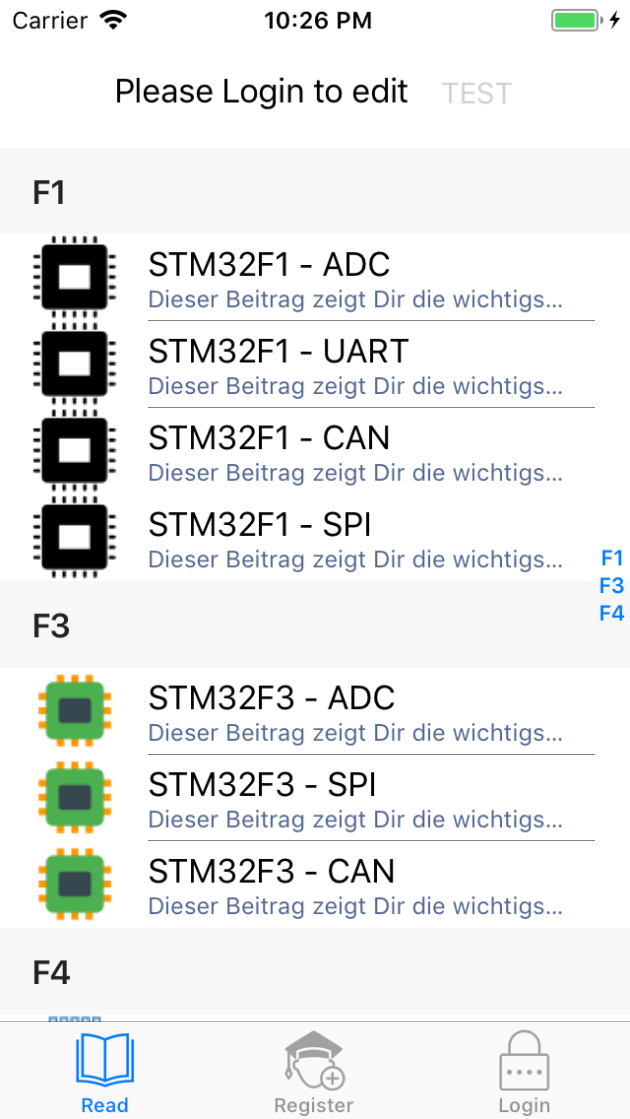
\includegraphics[width=.3\textwidth]{images/MCKB-iOS-Reading-Final.png}
		\end{subfigure}
		\begin{subfigure}
			\centering
			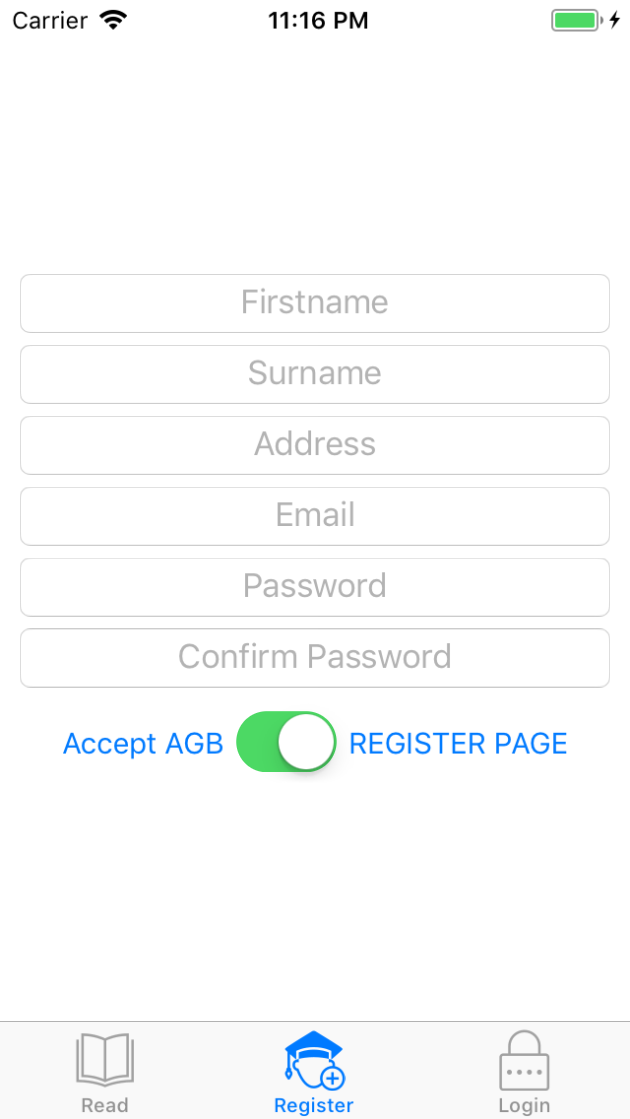
\includegraphics[width=.3\textwidth]{images/MCKB-iOS-Register-Final.png}
		\end{subfigure}
		\begin{subfigure}
			\centering
			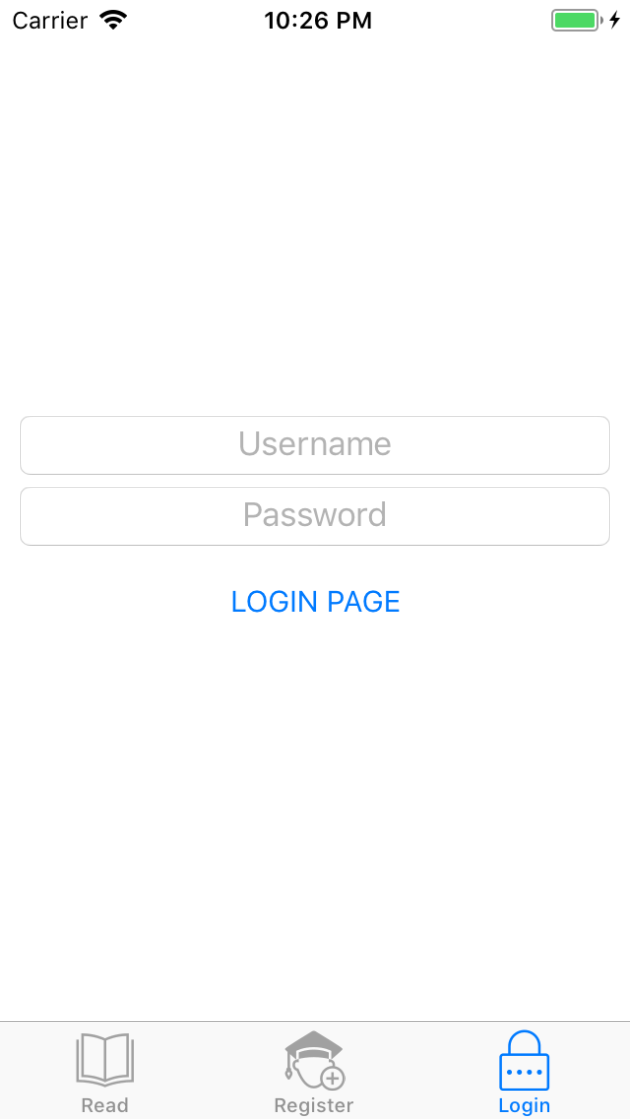
\includegraphics[width=.3\textwidth]{images/MCKB-iOS-Login-Final.png}
		\end{subfigure}
		\begin{subfigure}
			\centering
			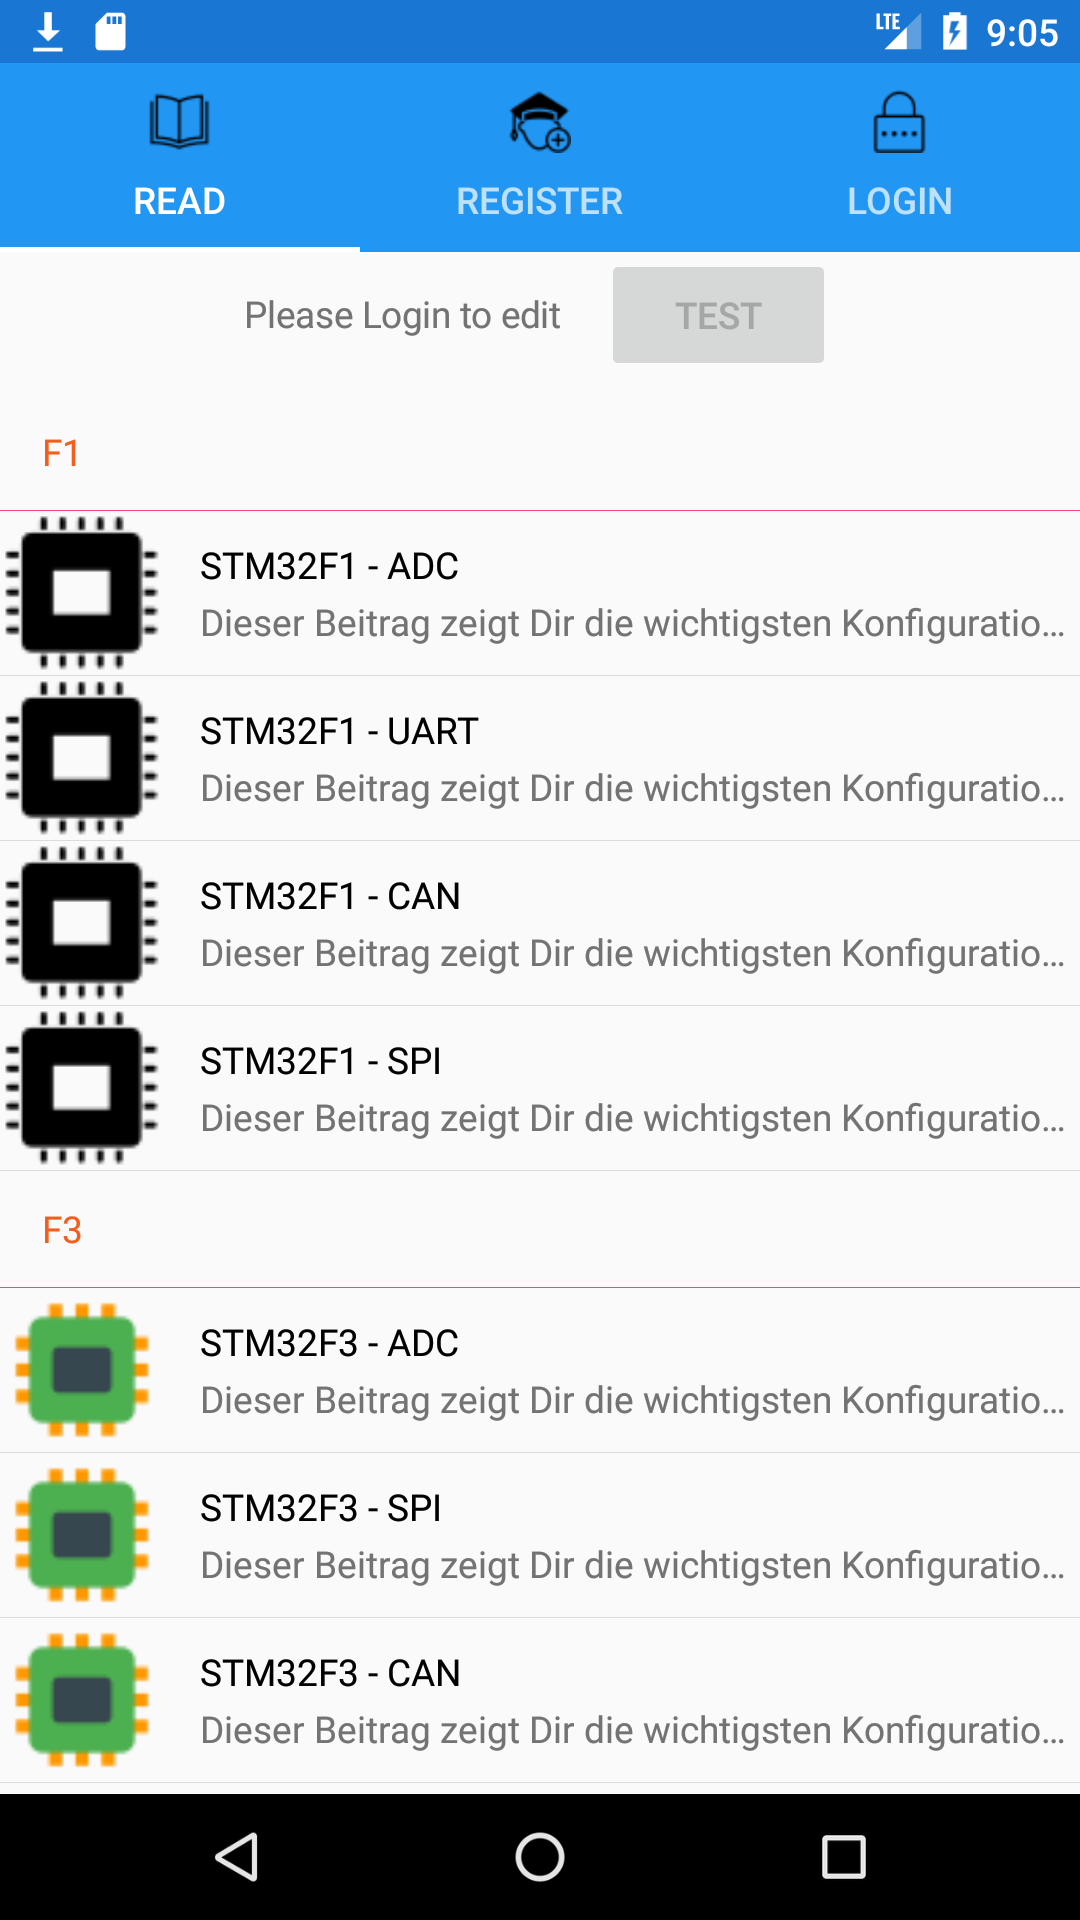
\includegraphics[width=.3\textwidth]{images/MCKB-Droid-Reading-Final.png}
		\end{subfigure}
		\begin{subfigure}
			\centering
			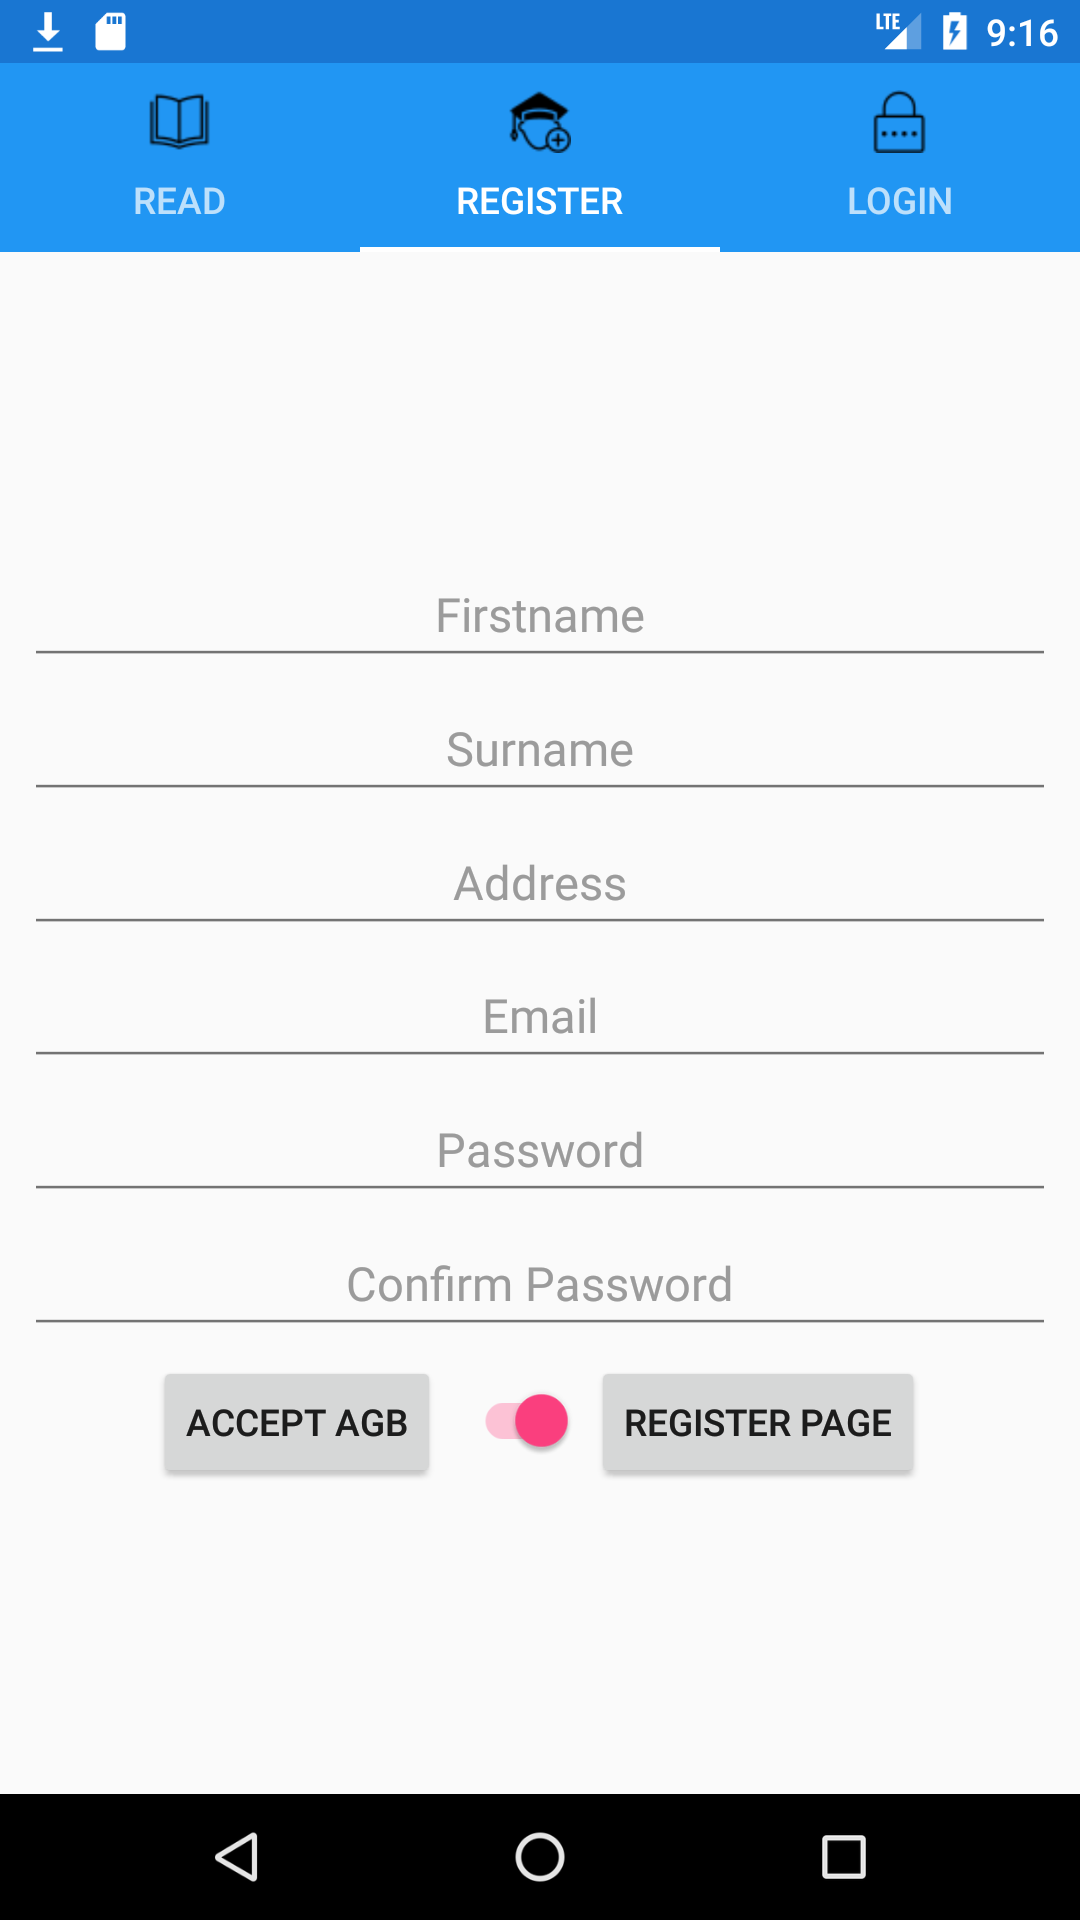
\includegraphics[width=.3\textwidth]{images/MCKB-Droid-Register-Final.png}
		\end{subfigure}
		\begin{subfigure}
			\centering
			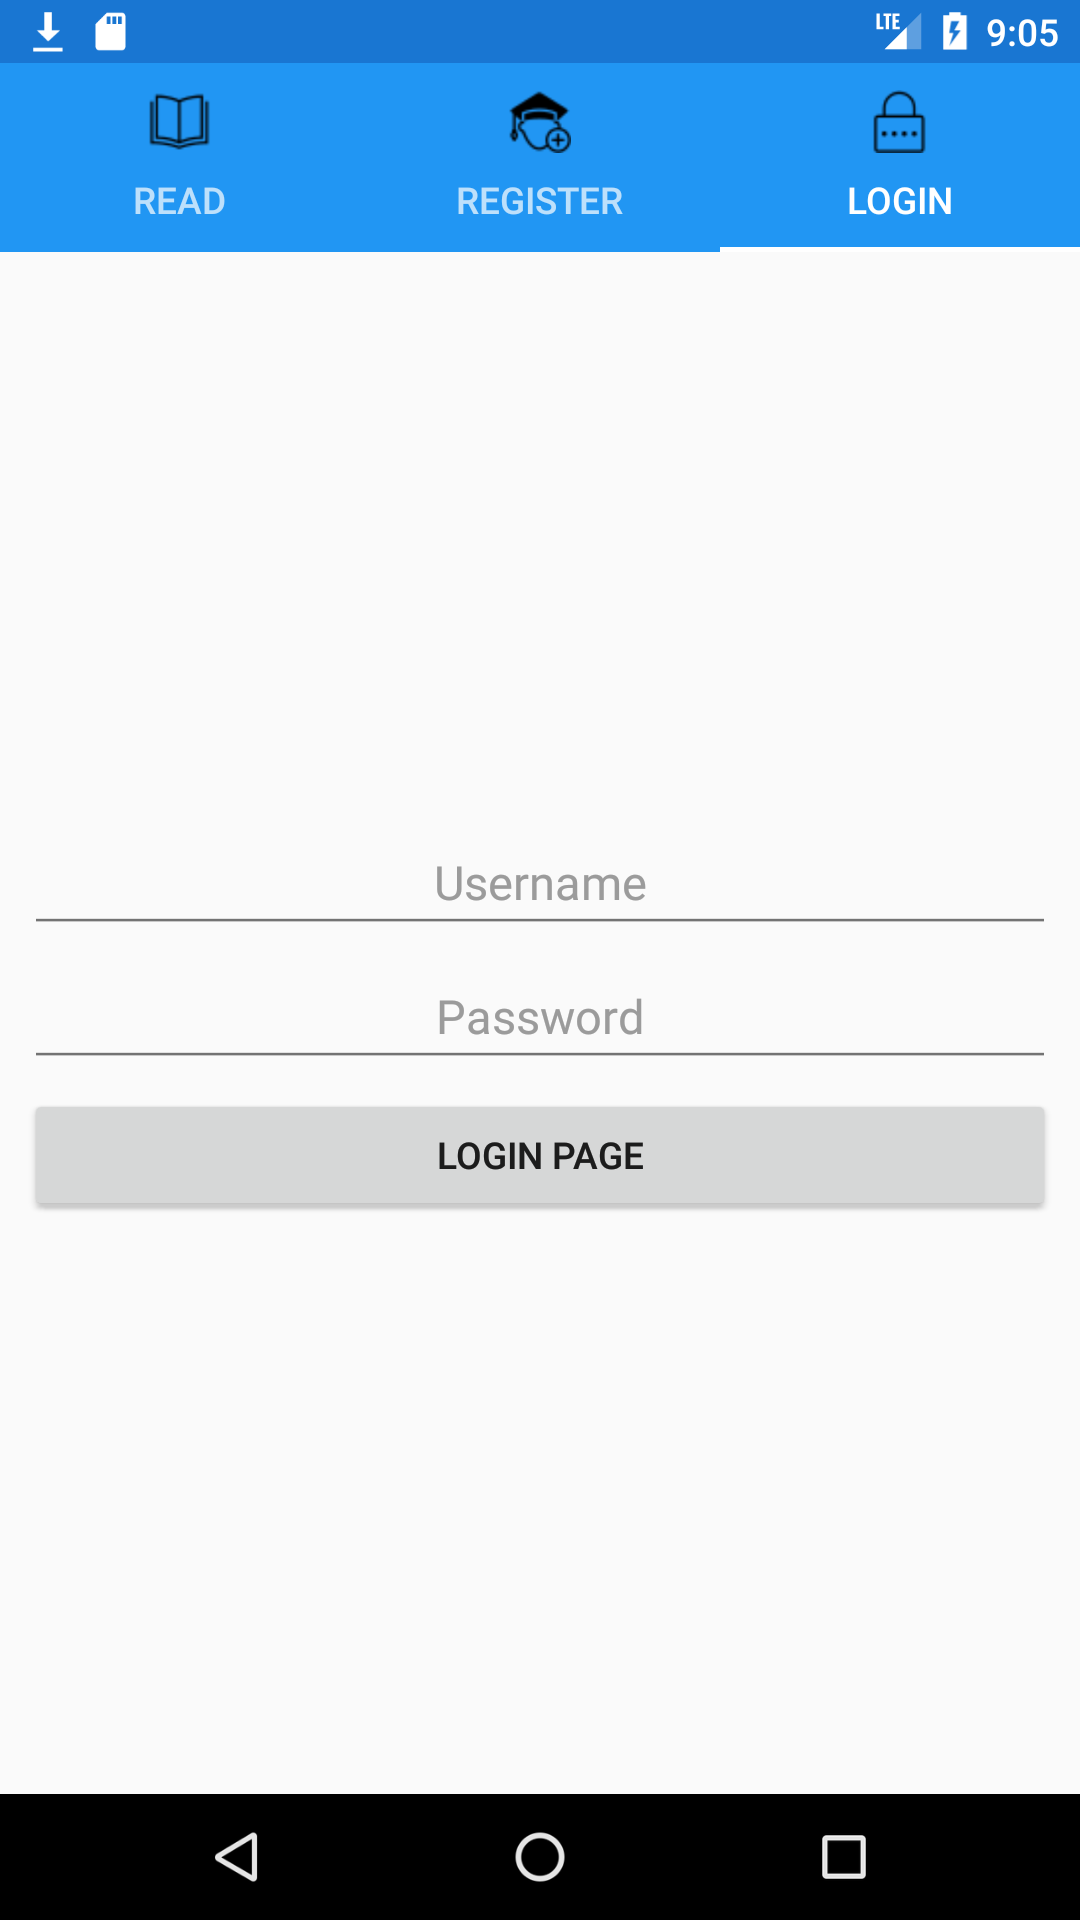
\includegraphics[width=.3\textwidth]{images/MCKB-Droid-Login-Final.png}
		\end{subfigure}
		\caption{Finales Design der MCKB App - Oben iOS / Unten Android}
		\label{fig:mckbAppfinal}
	\end{figure}
	
	\newpage
	\begin{lstlisting}[caption={MCKB - Design XAML Code},label={lst:mckbdesigncode},captionpos=b,style=XML-Own]
<?xml version="1.0" encoding="UTF-8"?>
<TabbedPage xmlns="http://xamarin.com/schemas/2014/forms" xmlns:x="http://schemas.microsoft.com/winfx/2009/xaml" x:Class="MCKB.MainPage">
    <!--Tabbed Page one is for the Artilces -->
    <ContentPage Title="Read" Icon="openbook.png">
        <ContentPage.Padding>
            <OnPlatform x:TypeArguments="Thickness" iOS="0,20,0,0" Android="0,0,0,0"></OnPlatform>
        </ContentPage.Padding>
        <StackLayout>
            <!--On top of the ListView to provide EDIT function -->
            <StackLayout>
                <StackLayout HorizontalOptions="Center" VerticalOptions="CenterAndExpand" Orientation="Horizontal">
                    <StackLayout.Padding>
                        <OnPlatform x:TypeArguments="Thickness" iOS="0,5,0,0" Android="0,0,0,0"></OnPlatform>
                    </StackLayout.Padding>
                    <Label Text="Please Login to edit" VerticalOptions="Center" HorizontalOptions="StartAndExpand"/>
                    <Button Text="Edit" IsEnabled="false" x:Name="editButton" Margin="10,0,0,0" Clicked="editButtonClicked"/>
                </StackLayout>
            </StackLayout>
            <ListView x:Name="articleListView" IsGroupingEnabled="true" GroupDisplayBinding="{Binding Title}">
                <ListView.ItemTemplate>
                    <DataTemplate>
                        <ImageCell Text="{Binding Title}" TextColor="Black" Detail="{Binding Description}" ImageSource="{Binding ImageUrl}"></ImageCell>
                    </DataTemplate>
                </ListView.ItemTemplate>
                <ListView.GroupHeaderTemplate>
                    <DataTemplate>
                        <TextCell Text="{Binding Title}" Detail="{Binding Description}" TextColor="#f35e20" DetailColor="#503026" />
                    </DataTemplate>
                </ListView.GroupHeaderTemplate>
            </ListView>
        </StackLayout>
    </ContentPage>

    <!--Tabbed Page two is for the registration of an user -->
    <ContentPage Title="Register" Icon="icons8studentregistrationfilled.png">
        <ContentPage.Padding>
            <OnPlatform x:TypeArguments="Thickness" iOS="0,20,0,0" Android="0,0,0,0"></OnPlatform>
        </ContentPage.Padding>
        <StackLayout HorizontalOptions="FillAndExpand" VerticalOptions="Center" Padding="10,10,10,10">
            <Entry HorizontalTextAlignment="Center" Placeholder="Firstname" x:Name="regfirstname"/>
            <Entry HorizontalTextAlignment="Center" Placeholder="Surname" x:Name="regsurname"/>
            <Entry HorizontalTextAlignment="Center" Placeholder="Address" x:Name="regaddress"/>
            <Entry HorizontalTextAlignment="Center" Placeholder="Email" x:Name="regemail" Keyboard="Email"/>
            <Entry HorizontalTextAlignment="Center" Placeholder="Password" x:Name="regpassword" IsPassword="true"/>
            <Entry HorizontalTextAlignment="Center" Placeholder="Confirm Password" x:Name="regconfpassword" IsPassword="true"/>
            <StackLayout HorizontalOptions="Center" VerticalOptions="CenterAndExpand">
                <StackLayout Orientation="Horizontal" Padding="0,0,0,0">
                    <Button Text="Accept AGB" VerticalOptions="Center" Clicked="showAgb"/>
                    <Switch IsToggled="false" x:Name="accept" VerticalOptions="Center"/>
                    <Button Text="REGISTER PAGE" IsEnabled="{Binding Source={x:Reference accept}, Path=IsToggled}" Clicked="sendRegistration"/>
                </StackLayout>
            </StackLayout>
        </StackLayout>
    </ContentPage>

    <!--Tabbed Page three is for the login -->
    <ContentPage Title="Login" Icon="icons8password.png">
        <ContentPage.Padding>
            <OnPlatform x:TypeArguments="Thickness" iOS="0,20,0,0" Android="0,0,0,0"></OnPlatform>
        </ContentPage.Padding>
        <StackLayout HorizontalOptions="FillAndExpand" VerticalOptions="Center" Padding="10,10,10,10">
            <Entry HorizontalTextAlignment="Center" Placeholder="Username" Keyboard="Text" x:Name="username"/>
            <Entry HorizontalTextAlignment="Center" Placeholder="Password" IsPassword="true" x:Name="password"/>
            <Button Text="LOGIN PAGE" Clicked="sendLogin"/>
        </StackLayout>
    </ContentPage>
</TabbedPage>
	\end{lstlisting}

% section zusätzliche_screenshots (end)



% (Hier können Schaltpläne, Programme usw. eingefügt werden.)
% Hier werden die Entwürfe zur Design der App gelistet sein.b
\clearpage

% --- List of Figures ----------------------------------------------------

\addcontentsline{toc}{section}{Abbildungsverzeichnis}
\listoffigures

\clearpage

% --- List of Tables -----------------------------------------------------

\addcontentsline{toc}{section}{Codeverzeichnis}
\lstlistoflistings

\addcontentsline{toc}{section}{Tabellenverzeichnis}
\listoftables

\clearpage

% --- Bibliography ------------------------------------------------------

\bibliographystyle{alpha}


% List references I definitely want in the bibliography,
% regardless of whether or not I cite them in the thesis.

\nocite{book:Xamarin.Forms-Succinctly}
\nocite{book:Xamarin.Forms-Essentials:}
\nocite{book:Cross-platform-UI-Development-with-Xamarin.Forms}
\nocite{book:Xamarin-Mobile-Application-Development}
\nocite{Amer2016}
\nocite{Oleksandr2015}
\nocite{8016193}
\nocite{Mukesh2016}
\nocite{Soylemez2017}
\nocite{Maximilian2017}

\addcontentsline{toc}{section}{Literaturverzeichnis}
\bibliography{thesis}

          % Appendix A

\end{document}

